\documentclass{article}

  % packages
    % basic stuff for rendering math
    \usepackage[letterpaper, top=1in, bottom=1in, left=1in, right=1in]{geometry}
    \usepackage[utf8]{inputenc}
    \usepackage[english]{babel}
    \usepackage{amsmath, amssymb} 
    \usepackage{bbm}              % for mathbbm

    % extra math symbols and utilities
    \usepackage{mathtools}        % for extra stuff like \coloneqq
    \usepackage{mathrsfs}         % for extra stuff like \mathsrc{}
    \usepackage{centernot}        % for the centernot arrow 
    \usepackage{bm}               % for better boldsymbol/mathbf 
    \usepackage{enumitem}         % better control over enumerate, itemize
    \usepackage{xr-hyper}
    \usepackage{hyperref}         % for hypertext linking
    \usepackage{fancyvrb}          % for better verbatim environments
    \usepackage{newverbs}         % for texttt{}
    \usepackage{xcolor}           % for colored text 
    \usepackage{listings}         % to include code
    \usepackage{lstautogobble}    % helper package for code
    \usepackage{parcolumns}       % for side by side columns for two column code
    

    % page layout
    \usepackage{fancyhdr}         % for headers and footers 
    \usepackage{lastpage}         % to include last page number in footer 
    \usepackage{parskip}          % for no indentation and space between paragraphs    
    \usepackage[T1]{fontenc}      % to include \textbackslash
    \usepackage{footnote}
    \usepackage{etoolbox}

    % for custom environments
    \usepackage{tcolorbox}        % for better colored boxes in custom environments
    \tcbuselibrary{breakable}     % to allow tcolorboxes to break across pages

    % figures and tables 
    \usepackage{pgfplots}
    \pgfplotsset{compat=1.18}
    \usepackage{float}            % for [H] figure placement
    \usepackage{tikz, tikz-cd}
    \usetikzlibrary{arrows, positioning, calc}
    \usepackage{graphicx}
    \usepackage{caption, subcaption} 
    \usepackage{dcolumn}

    \usepackage[nottoc]{tocbibind}
    \pdfsuppresswarningpagegroup=1
    \hfuzz=5.002pt                % ignore overfull hbox badness warnings below this limit

  % New and replaced operators
    \DeclareMathOperator{\std}{std}
    \DeclareMathOperator*{\argmin}{\arg\!\min}
    \DeclareMathOperator*{\argmax}{\arg\!\max}
    \newcommand{\ket}[1]{\ensuremath{\left|#1\right\rangle}}
    \newcommand{\bra}[1]{\ensuremath{\left\langle#1\right|}}
    \newcommand{\braket}[2]{\langle #1 | #2 \rangle}
    \newcommand{\qed}{$\blacksquare \quad$}     % I like QED squares to be black

  % Custom Environments
    \tcbset{
      colframe = black,
      colback  = white,
      coltitle = black,
      colbacktitle = black!10,
      breakable, 
      arc=0mm,
      boxrule=1pt,
      left=8pt,
      right=8pt,
      top=6pt,
      bottom=6pt,
      before skip=12pt,
      after skip=12pt,
      bottomrule at break=-1pt,
      toprule at break=-1pt,
      fonttitle=\bfseries,
    }
    \newcounter{question}[section]
    \renewcommand{\thequestion}{\thesection.\arabic{question}}
    \NewDocumentEnvironment{question}{O{} o}{%
      \refstepcounter{question}%
      \ifstrempty{#1}{%
        \begin{tcolorbox}[title=\textbf{Question \thequestion}]%
      }{%
        \IfValueTF{#2}{%
          \begin{tcolorbox}[title=\textbf{Question \thequestion~(#1)}, label={#2}]%
        }{%
          \begin{tcolorbox}[title=\textbf{Question \thequestion~(#1)}]%
        }%
      }%
    }{%
      \end{tcolorbox}%
    }

    \newcounter{exercise}[section]
    \renewcommand{\theexercise}{\thesection.\arabic{exercise}}
    \NewDocumentEnvironment{exercise}{O{} o}{%
      \refstepcounter{exercise}%
      \ifstrempty{#1}{%
        \begin{tcolorbox}[title=\textbf{Exercise \theexercise}]%
      }{%
        \IfValueTF{#2}{%
          \begin{tcolorbox}[title=\textbf{Exercise \theexercise~(#1)}, label={#2}]%
        }{%
          \begin{tcolorbox}[title=\textbf{Exercise \theexercise~(#1)}]%
        }%
      }%
    }{%
      \end{tcolorbox}%
    }

    \newtcolorbox[auto counter, number within=section]{solution}[1][]
    {
      before skip = -7pt,
      before upper = \textit{Solution. },
    }

    \newcounter{theorem}[section]
    \renewcommand{\thetheorem}{\thesection.\arabic{theorem}}

    \NewDocumentEnvironment{lemma}{O{} o}{%
      \refstepcounter{theorem}%
      \ifstrempty{#1}{%
        \begin{tcolorbox}[title=\textbf{Lemma \thetheorem}]%
      }{%
        \IfValueTF{#2}{%
          \begin{tcolorbox}[title=\textbf{Lemma \thetheorem~(#1)}, label={#2}]%
        }{%
          \begin{tcolorbox}[title=\textbf{Lemma \thetheorem~(#1)}]%
        }%
      }%
    }{%
      \end{tcolorbox}%
    }

    \NewDocumentEnvironment{theorem}{O{} o}{%
      \refstepcounter{theorem}%
      \ifstrempty{#1}{%
        \begin{tcolorbox}[title=\textbf{Theorem \thetheorem}]%
      }{%
        \IfValueTF{#2}{%
          \begin{tcolorbox}[title=\textbf{Theorem \thetheorem~(#1)}, label={#2}]%
        }{%
          \begin{tcolorbox}[title=\textbf{Theorem \thetheorem~(#1)}]%
        }%
      }%
    }{%
      \end{tcolorbox}%
    }

    \NewDocumentEnvironment{corollary}{O{} o}{%
      \refstepcounter{theorem}%
      \ifstrempty{#1}{%
        \begin{tcolorbox}[title=\textbf{Corollary \thetheorem}]%
      }{%
        \IfValueTF{#2}{%
          \begin{tcolorbox}[title=\textbf{Corollary \thetheorem~(#1)}, label={#2}]%
        }{%
          \begin{tcolorbox}[title=\textbf{Corollary \thetheorem~(#1)}]%
        }%
      }%
    }{%
      \end{tcolorbox}%
    }

    \newtcolorbox[auto counter, number within=section]{proof}[1][]
    {
      before skip = -7pt,
      before upper = \textit{Proof. },
    }

    \newcounter{definition}[section]
    \renewcommand{\thedefinition}{\thesection.\arabic{definition}}
    \NewDocumentEnvironment{definition}{O{} o}{%
      \refstepcounter{definition}%
      \ifstrempty{#1}{%
        \begin{tcolorbox}[title=\textbf{Definition \thedefinition}]%
      }{%
        \IfValueTF{#2}{%
          \begin{tcolorbox}[title=\textbf{Definition \thedefinition~(#1)}, label={#2}]%
        }{%
          \begin{tcolorbox}[title=\textbf{Definition \thedefinition~(#1)}]%
        }%
      }%
    }{%
      \end{tcolorbox}%
    }

    \newcounter{example}[section]
    \renewcommand{\theexample}{\thesection.\arabic{example}}
    \NewDocumentEnvironment{example}{O{} o}{%
      \refstepcounter{example}%
      \ifstrempty{#1}{%
        \begin{tcolorbox}[title=\textbf{Example \theexample}]%
      }{%
        \IfValueTF{#2}{%
          \begin{tcolorbox}[title=\textbf{Example \theexample~(#1)}, label={#2}]%
        }{%
          \begin{tcolorbox}[title=\textbf{Example \theexample~(#1)}]%
        }%
      }%
    }{%
      \end{tcolorbox}%
    }

    \newcounter{code}[section]
    \renewcommand{\thecode}{\thesection.\arabic{code}}
    \NewDocumentEnvironment{code}{O{} o}{%
      \refstepcounter{code}%
      \ifstrempty{#1}{%
        \begin{tcolorbox}[title=\textbf{Code \thecode}]%
      }{%
        \IfValueTF{#2}{%
          \begin{tcolorbox}[title=\textbf{Code \thecode~(#1)}, label={#2}]%
        }{%
          \begin{tcolorbox}[title=\textbf{Code \thecode~(#1)}]%
        }%
      }%
    }{%
      \end{tcolorbox}%
    } 

    \definecolor{dkgreen}{rgb}{0,0.6,0}
    \definecolor{gray}{rgb}{0.5,0.5,0.5}
    \definecolor{mauve}{rgb}{0.58,0,0.82}
    \definecolor{lightgray}{gray}{0.93}

    % default options for listings (for code)
    \lstset{
      autogobble,
      frame=ltbr,
      language=C,                           % the language of the code
      aboveskip=3mm,
      belowskip=3mm,
      showstringspaces=false,
      columns=fullflexible,
      keepspaces=true,
      basicstyle={\small\ttfamily},
      numbers=left,
      firstnumber=1,                        % start line number at 1
      numberstyle=\tiny\color{gray},
      keywordstyle=\color{blue},
      commentstyle=\color{dkgreen},
      stringstyle=\color{mauve},
      backgroundcolor=\color{lightgray}, 
      breaklines=true,                      % break lines
      breakatwhitespace=true,
      tabsize=3, 
      xleftmargin=2em, 
      framexleftmargin=1.5em, 
      stepnumber=1
    }

  % Page style
    \pagestyle{fancy}
    \fancyhead[L]{Measure Theory}
    \fancyhead[C]{Muchang Bahng}
    \fancyhead[R]{Fall 2025} 
    \fancyfoot[C]{\thepage / \pageref{LastPage}}
    \renewcommand{\footrulewidth}{0.4pt}          % the footer line should be 0.4pt wide
    \renewcommand{\thispagestyle}[1]{}  % needed to include headers in title page

  % external documents 
   \externaldocument[real-]{../Univariate_Analysis/paper}[../Univariate_Analysis/paper.pdf] 
   \externaldocument[set-]{../Set_Theory/paper}[../Set_Theory/paper.pdf] 

\begin{document}

\title{Measure Theory}
\author{Muchang Bahng}
\date{Fall 2025}

\maketitle
\tableofcontents
\pagebreak

Unlike my machine learning notes, which focuses mostly on the theoretical soundness of classical (e.g. pre-deep and interpretable) models, the theory of deep neural networks have not been developed as well yet. Furthermore, the recency of developments, especially in the post-2010s, results in a pretty nonlinear\footnote{No pun intended.} timeline that is difficult to categorize effectively. Before I give my motivation, the direct prerequisites for deep learning are basic knowledge of my notes in probability theory, machine learning, and real analysis. 

Therefore, after much thought, I think organizing my notes in chronological order would be best. It turned out that in the early days of deep learning, most researchers like Andrew Ng stated that he focused on supervised models,\footnote{He states this in his podcast with Lex Fridman.} and it wasn't until the 2010s that the development of unsupervised models burgeoned. 

\begin{enumerate}
  \item We start by introducing \textit{multilayered perceptrons} (MLPs), which build upon generalized linear models (GLMs) that we have went over in machine learning. This is pretty much the ``foundational'' model that we will build on. We then talk a about practical methodologies regarding training and control. 

  \item Then we introduce the other two architectures. The \textit{convolutional neural network} (CNN) gives us a scalable way to perform sparse matrix multiplication efficiently, by taking advantage of locality. Then in \textit{recurrent neural networks} (RNNs), we are not limited to a single $n$-dimensional vector input and are able to process a time series of inputs.  
    
  \item With these building blocks, we are able take and two neural networks together to create an encoder-decoder model. The two main applications of this was dimensionality reduction with \textit{autoencoders}, followed by \textit{seq2seq} for machine translation between sequences of words.  

  \item The practical success of autoencoders led to the development of not just density estimation models, but \textit{generative} ones that seek to sample from the learned distribution. These generative models were ``deep'' extensions of the classical linear factor models resulting in \textit{restricted Boltzmann machines (RBMs)} and \textit{variational autoencoders (VAEs)}, which attempted to explicitly model an approximation of the true data generating distribution. More specifically, RBMs were \textit{energy models} that borrowed ideas from physics to learn a distribution of the form $p_X (x) = \frac{1}{Z} e^{-f_\theta (x)}$. To sample from this, researchers already had access to the established Markov Chain Monte Carlo (MCMC) algorithms designed for this exact problem. As for VAEs, these were trained and sampled through \textit{variational inference} methods. 

  \item In 2014, a completely new architecture composed of 2 neural networks competing each other gave rise to \textit{generative adversarial networks} (GANs) which blew RBMs and VAEs away. A similar architecture followed with \textit{generative stochastic networks} (GSNs).

  \item In 2016, \textit{normalizing flow models}, which attempted to model a smooth function that transformed simple latent variables to the true data generating distribution, were invented by Google DeepMind and surpassed GANs. 

  \item In 2017, \textit{attention} took the world by storm, which had drastically improved machine translation in seq2seq, and the resulting \textit{self-attention} plus the \textit{transformer} architectures led to the success of OpenAI's ChatGPT. 
\end{enumerate} 

Again, I emphasize that the math in these notes are not very advanced. However, implementing these simple models and training algorithms from scratch is a challenge in itself. I will go through implementing everything from scratch as if we were building a mini-version of PyTorch as we learn new topics. My implementations can be found \href{https://github.com/mbahng/pyember}{here}. 

\section{Jordan Measure}

  We would like to generalize the concepts of size, which are specified as length/area/volume depending on the dimension of the space we live in. The most intuitive notion of size are those of segments, rectangles, and boxes, and these are the simplest forms of sets that we will work with. 

  Such that for ``simple'' sets $A$ where we know what the area is, the outer measure of $A$ should coincide with the area of $A$. Let's first start by defining what a ``simple'' set is. 

  \begin{definition}[Box] 
    An \textbf{box} $E \subset \mathbb{R}^n$ is defined recursively as follows. 
    \begin{enumerate}
      \item An \textbf{interval} $I \subset \mathbb{R}$ is one of the sets $(a, b), [a, b), (a, b], [a, b]$ for $a, b \in \mathbb{R}$. 
      \item For $n > 1$, an box $E \subset \mathbb{R}^n$ is $E = I_1 \times \ldots \times I_n$ for intervals $I_1, \ldots, I_k$. 
    \end{enumerate}
  \end{definition} 

  \begin{definition}[Size of a Box]
    The \textbf{size} of a box $E = I_1 \times \ldots \times I_n \subset \mathbb{R}^n$ is defined as follows. 
    \begin{enumerate}
      \item The \textbf{length} of an interval $I$ is $\ell(I) \coloneqq b - a$. 
      \item The \textbf{size} of $E$ is $|E| \coloneqq \prod_{i=1}^n (b_i - a_i)$. 
    \end{enumerate}
  \end{definition} 

  Now we can combine these to get an elementary set. 

  \begin{definition}[Elementary Set]
    An \textbf{elementary set} is a set $E \subset \mathbb{R}^n$ that is a finite union of boxes. 
  \end{definition}

  We would like to have some nice properties of these elementary sets. 

  \begin{lemma}[Boolean Closure of Elementary Sets]
    Given two elementary sets $E, F \subset \mathbb{R}^n$, 
    \begin{enumerate}
      \item $E \cup F$ is elementary. 
      \item $E \cap F$ is elementary. 
      \item $E \setminus F$ is elementary. 
    \end{enumerate}
  \end{lemma}
  \begin{proof}
    
  \end{proof}

  \begin{lemma}[Disjoint Finite Union of Elementary Sets]
    Let $E \subset \mathbb{R}^n$ be an elementary set. Then, $E$ can be expressed as a finite union of \textit{disjoint} boxes. 
  \end{lemma}
  \begin{proof}
    
  \end{proof}

  \begin{definition}[Elementary Measure]
    The \textbf{elementary measure} of an elementary set $E \subset \mathbb{R}^n$ is defined as the sum of the sizes of each box in a partition: 
    \begin{equation}
      m(E) \coloneqq \sum_{i=1}^k |B_k|
    \end{equation}
    We claim that this sum is invariant depending on the partition, and hence, well defined. 
  \end{definition}
  \begin{proof}
    
  \end{proof}

  This elementary measure clearly extends the notion of size, since 
  \begin{equation}
    m(B) = s(B)
  \end{equation}
  whenever $B$ is elementary. Furthermore, we can deduce finite additivity and nonnegativity. These are really trivial but we state them as theorems to establish a pattern. 

  \begin{lemma}[Fundamental Properties of Elementary Measure]
    The elementary measure satisfies the following. 
    \begin{enumerate}
      \item \textit{Nonnegativity}. For any elementary set $E$, $m(E) \geq 0$. 
      \item \textit{Finite Additivity} Given $E_1, \ldots, E_n$ are disjoint elementary sets, 
      \begin{equation}
        m(E_1 \cup \ldots \cup E_k) = m(E_1) + \ldots + m(E_k)
      \end{equation}

      \item \textit{Monotonicity}. Given elementary sets $E \subset F$, we have 
      \begin{equation}
        m(E) \leq m(F)
      \end{equation}

      \item \textit{Finite Subadditivity}. Let $E_1, \ldots, E_n$ be any elementary sets (not necessarily disjoint). Then 
      \begin{equation}
        m(E_1 \cup \ldots \cup E_n) \leq m(E_1) + \ldots + m(E_n)
      \end{equation}

      \item \textit{Translation Invariance}. For $x \in \mathbb{R}^n$ and elementary set $E \subset \mathbb{R}^n$, 
      \begin{equation}
        m(E) = m(x + E) 
      \end{equation}
    \end{enumerate}
  \end{lemma}

  It turns out that these properties uniquely determine an elementary measure. 

  \begin{theorem}[Uniqueness of Elementary Measure]
    
  \end{theorem}

\subsection{Jordan Measure}

  Now, we define the outer and inner measure, which are defined for \textit{all} subsets of $\mathbb{R}^n$. 

  \begin{definition}[Jordan Outer, Inner Measure]
    Let $E \subset \mathbb{R}^n$. 
    \begin{enumerate}
      \item The \textbf{Jordan inner measure} is defined 
      \begin{equation}
        m_\ast (E) \coloneqq \sup_{A \subset E, A \text{ elementary}} m(A)
      \end{equation}

      \item The \textbf{Jordan outer measure} is defined 
      \begin{equation}
        m_\ast (E) \coloneqq \inf_{B \supset E, B \text{ elementary}} m(B)
      \end{equation}
    \end{enumerate}
    Note that if $E$ is unbounded, then there exists no elementary set that is a superset of $E$, and so the infimum of such a set is $+\infty$ conventionally. 
  \end{definition}

  This is where our first big leap in construction comes in. Before, we have defined elementary boxes, which are pretty much guaranteed to have a well-defined elementary measure. Here, we \textit{begin} with a function on the power set of $\mathbb{R}^n$, and then we will filter the power set to those subsets that behave nicely. 

  \begin{definition}[Jordan Measurable Set, Jordan Measure]
    Let $E \subset \mathbb{R}^n$ be bounded.\footnote{Note that by convention, we don't consider unbounded sets to be Jordan measurable.} If $m_\ast (E) = m^\ast (E)$, then $E$ is said to be \textbf{Jordan-measurable}, and we define 
    \begin{equation}
      m(E) \coloneqq m_\ast (E) = m^\ast (E)
    \end{equation}
    as the \textbf{Jordan measure} of $E$. 
  \end{definition}

  Note first of all that Jordan measure is a generalization of elementary measure, since if $E$ is elementary, then we can set $A = E = B$ to achieve these bounds. Furthermore, by monotonicity, we can never get past them, and will always have 
  \begin{equation}
    m(A) \leq m(E) \leq m(B)
  \end{equation}
  where $m$ is the elementary measure. So, we can overload the notation and just write $m$ to denote elementary and Jordan measure. Second, note that the Jordan measure shares the same properties. 

  \begin{lemma}[Boolean Closure of Jordan Measurable Sets]
    Given two Jordan-measurable sets $E, F \subset \mathbb{R}^n$, 
    \begin{enumerate}
      \item $E \cup F$ is elementary. 
      \item $E \cap F$ is elementary. 
      \item $E \setminus F$ is elementary. 
    \end{enumerate}
  \end{lemma}
  \begin{proof}
    
  \end{proof}

  The properties of the Jordan measure parallel those of elementary measure. 

  \begin{theorem}[Fundamental Properties of Jordan Measure]
    The elementary measure satisfies the following. 
    \begin{enumerate}
      \item \textit{Nonnegativity}. For any elementary set $E$, $m(E) \geq 0$. 
      \item \textit{Finite Additivity} Given $E_1, \ldots, E_n$ are disjoint elementary sets, 
      \begin{equation}
        m(E_1 \cup \ldots \cup E_k) = m(E_1) + \ldots + m(E_k)
      \end{equation}

      \item \textit{Monotonicity}. Given elementary sets $E \subset F$, we have 
      \begin{equation}
        m(E) \leq m(F)
      \end{equation}

      \item \textit{Finite Subadditivity}. Let $E_1, \ldots, E_n$ be any elementary sets (not necessarily disjoint). Then 
      \begin{equation}
        m(E_1 \cup \ldots \cup E_n) \leq m(E_1) + \ldots + m(E_n)
      \end{equation}

      \item \textit{Translation Invariance}. For $x \in \mathbb{R}^n$ and elementary set $E \subset \mathbb{R}^n$, 
      \begin{equation}
        m(E) = m(x + E) 
      \end{equation}
    \end{enumerate}
  \end{theorem}
  \begin{proof}
    
  \end{proof}

  Jordan measurable sets are sets that are ``almost'' elementary, but a few sets already come to mind that are not Jordan measurable. 

  \begin{example}[Rationals in Unit Interval]
    $\mathbb{Q} \cap [0, 1]$ is not Jordan measurable. 
  \end{example} 

  It may be hard to tell directly whether something is Jordan measurable. This is where the ``Cauchy criterion'' of Jordan measurable sets comes in. 

  \begin{theorem}[Equivalent Notions]
    $E$ is Jordan measurable iff $\forall \epsilon > 0$, $\exists$ elementary sets $A \subset E \subset B$ s.t. $m(B \setminus A) < \epsilon$. 
  \end{theorem}
  \begin{proof}
    
  \end{proof}

  Note how the previous lemma is very similar to \hyperref[real-thm:cauchy-riemann-integrability]{this theorem on Riemann integrability}. 

  \begin{example}[Regions Under Graphs are Jordan Measurable]
    
  \end{example}

  \begin{example}[Triangle is Jordan Measurable]
    
  \end{example}

  \begin{example}[Compact Convex Polytopes are Jordan Measurable]
    
  \end{example}

  \begin{example}[Open and Closed Balls in Euclidean Space are Jordan Measurable]
    
  \end{example}

  \begin{example}[Subsets of Jordan Null Sets have 0 Jordan Measure]
    
  \end{example}

  \begin{theorem}[Uniqueness of Jordan Measure]
    
  \end{theorem}

  \begin{theorem}[Topological Approximations of Jordan Measurable Sets]
    Let $E \subset \mathbb{R}^n$ be a bounded set. Then, 
    \begin{enumerate}
      \item $E$ and its closure $\overline{E}$ have the same Jordan outer measure. 
      \item $E$ and its interior $E^\circ$ have the same Jordan outer measure. 
      \item $E$ is Jordan measurable iff the topological boundary $\partial E$ has Jordan outer measure $0$. 
    \end{enumerate}
  \end{theorem}
  \begin{proof}
    
  \end{proof}

  \begin{example}[Bullet Riddled Square]
    Show that both sets have a Jordan inner measure $0$ and Jordan outer measure $1$. 
    \begin{enumerate}
      \item $[0, 1]^2 \setminus \mathbb{Q}^2$. 
      \item $[0, 1]^2 \cap \mathbb{Q}^2$. 
    \end{enumerate}
  \end{example}

  Finally, a little teaser theorem. 

  \begin{theorem}[Caratheodory Property]
    Let $E \subset \mathbb{R}^n$ be a bounded set, and $F \subset \mathbb{R}^n$ be an elementary set. Show that 
    \begin{equation}
      m^\ast (E) = m^\ast (E \cap F) + m^\ast(E \setminus F)
    \end{equation}
    where $m^\ast$ is the Jordan outer measure. 
  \end{theorem}
  \begin{proof}
    
  \end{proof}

\subsection{Riemann Integration} 

  Now, we connect the Riemann integral to the Jordan measure. 

  \begin{theorem}[Jordan Measure with Riemann Integral]
    If $E \subset [a, b]$ is Jordan measurable, then the indicator function $\mathbbm{1}_E$ is Riemann integrable, and 
    \begin{equation}
      \int_a^b \mathbbm{1}_{E} \,dx = m(E)
    \end{equation}
  \end{theorem}



\include{sec/lebesgue}
\section{Measurable Functions}

  So far, we have defined measurable sets, constructed the Lebesgue measure, and shown that Lebesgue measurable sets can be approximated by nice open sets. Now, let's talk about measurable functions. Just like for measurable sets, there is a general sense in which we can define them and there is the more ``Euclidean'' way of defining them. 

  \begin{definition}[Measurable Function]
    Given a measurable space $(X, \mathcal{A})$, $f: (X, \mathcal{A}) \longrightarrow \mathbb{R}$ is \textbf{measurable} if 
    \begin{equation}
      f^{-1}(A) \in \mathcal{A} \text{ for all } A \text{ open}
    \end{equation}
    Note that measurable functions are always defined on measurable sets, so we don't have to state that its domain is always measurable. 
  \end{definition}

  \begin{theorem}[Measurable Functions on Real Line]
    Let $f: E \subset \mathbb{R} \to \mathbb{R} \cup \{ \pm \infty\}$ and $E$ be measurable. Then, TFAE 
    \begin{enumerate} 
      \item $\forall c \in \mathbb{R}$, $\{x \in E \mid f(x) > c\}$ is measurable. 
      \item $\forall c \in \mathbb{R}$, $\{x \in E \mid f(x) \geq c\}$ is measurable. 
      \item $\forall c \in \mathbb{R}$, $\{x \in E \mid f(x) < c\}$ is measurable. 
      \item $\forall c \in \mathbb{R}$, $\{x \in E \mid f(x) \leq c\}$ is measurable. 
      \item $f$ is Lebesgue measurable. 
    \end{enumerate}
    Furthermore, if any of these hold, then also $\{x \in E \mid f(x) = c \}$ is measurable for all $c$ (but not the converse!). 
  \end{theorem} 
  \begin{proof}
    We know that $(1) \iff (4)$ and $(2) \iff (3)$ by taking complements. We prove $(1) \iff (2)$. 
    \begin{enumerate}
      \item $(1) \implies (2)$. 
      \begin{equation}
        \{x \in E \mid f(x) \geq c \} = \bigcap_{k=1}^\infty \{x \in E \mid f(x) > c - \frac{1}{k} \}
      \end{equation}

      \item $(2) \implies (1)$. 
      \begin{equation}
        \{ x \in E \mid f(x) > c\} = \bigcup_{k=1}^\infty \{x \in E \mid f(x) \geq c + \frac{1}{k} \}
      \end{equation}
    \end{enumerate}

    For $(5)$, we know that
    \begin{enumerate}
      \item $(5) \implies (1)$ is trivial, since open intervals are open sets. 
      \item $(1) \implies (5)$. Any open set is a countable union of disjoint open intervals, and so let 
      \begin{equation}
        U = \bigcup_{k=1}^\infty I_k, \qquad I_k = (a_k, b_k) = \underbrace{(-\infty, b_k)}_{B_k} \cap \underbrace{(a_k, +\infty)}_{A_k}
      \end{equation} 
      Therefore, 
      \begin{equation}
        f^{-1} (U) = \bigcup_{k=1}^\infty f^{-1} (B_k \cap A_k) = \bigcup_{k=1}^\infty \{f^{-1} (B_k) \cap f^{-1} (A_k) \}
      \end{equation}
      which is measurable since countable union/intersections are measurable (by definition of $\sigma$-algebra). 
    \end{enumerate}

    For the final implication, we can use $(2)$ and $(4)$ to get 
    \begin{equation}
      \{x \in E \mid f(x) = c\} = \{x \in E \mid f(x) \leq c \} \cup \{x \in E \mid f(x) \geq c \}
    \end{equation}
  \end{proof} 

  The first question is how you would relate this to continuity. 

  \begin{theorem}[Continuous Functions are Measurable]
    If $f: X \to \mathbb{R}$ is continuous, then it is measurable. 
  \end{theorem}
  \begin{proof}
    If $f$ is continuous, then $f^{-1} (O) = U \cap X$ for every open $O$ with open $U$. 
  \end{proof}

  \begin{theorem}[Monotonic Functions are Measurable] 
    Let $I$ be an interval. If $f: I \subset \mathbb{R}$ is monotone, then $f$ is measurable.
  \end{theorem}
  \begin{proof}
    You can probably see that it is more advantageous to prove using the definition of measurability using rays. We wish to show that for all $c$, $E_c \coloneqq \{x \in I \mid f(x) > c\}$ is measurable. We wish to show that $E_c$ is an interval, though there seems to be some complications with potential discontinuities. 

    Therefore, we use an equivalent definition of an interval: $I$ is an interval if for every $x, y \in I$, $x < t < y \implies t \in I$. Therefore, we can see that if $x, y \in E_c$, then $f(x) > c, f(y) > c$. Therefore, if $t$ is in between them, $f(t) > f(\min\{x, y\}) > c$, and so $t \in E_c$. Since intervals are measurable, we are done. 
  \end{proof}

  There is also some notion of robustness. 

  \begin{theorem}[Function Difference on Measure 0 Set Doesn't Affect Measurability]
    Suppose $f: E \subset \mathbb{R} \to \mathbb{R} \cup \{\pm \infty\}$ with $E$ measurable, and let $g$ be some other function. If $f$ is measurable on $E$ and $g(x) = f(x)$ a.e. for $x \in E$, then $g$ is measurable on $E$. 
  \end{theorem}
  \begin{proof}
    We wish to show that for any open $O \subset \mathbb{R}$, $g^{-1} (O)$ is measurable. We might start with Carathéodory and try to show that for all $A \subset E$, 
    \begin{equation}
      m^\ast(A) = m^\ast (A \cap g^{-1}(O)) + m^\ast (A \cap g^{-1}(O)^c)
    \end{equation}
    But this turns out to be overkill. Since this is about $0$ measure sets, you should be thinking about how $0$-measure sets do not affect measurability and try to use this. In $g^{-1}(O)$, there is a portion of it that overlaps with $f$---call it $A \subset E$---and a portion that doesn't. We know that $m^\ast (E \setminus A) = 0$\footnote{TBD: Can we write $m$? } and a measure $0$ set difference doesn't affect measurability, so $A$ is measurable. So let's decompose it. 
    \begin{align}
      g^{-1} (O) & = \big( g^{-1} (O) \cap A \big) \cup \big( g^{-1} (O) \cap (E \setminus A) \big) \\ 
                 & = \big( f^{-1} (O) \cap A \big) \cup \big( g^{-1} (O) \cap (E \setminus A) \big)
    \end{align}
    If we try to take the measure of this, the first term is the union of measurable sets $f^{-1} (O)$ and $A$. The second term is also measurable since the outer measure is $0$, by subadditivity compared to $m^\ast(E \setminus A) = 0$. Therefore $g^{-1} (O)$ is measurable. 
  \end{proof}
  \begin{proof}
    In class. Consider $S = \{x \in E \mid g(x) < c \}$. Let $A \subset E$ be the set where $g(x) = f(x)$, with $m (E \setminus A) = 0$. Then, 
    \begin{equation}
      S = \big( \{x \in E \mid g(x) < c\} \cap (E \setminus A) \big) \cup \big( \{x \in E \mid f(x) < c\} \cap A \big) 
    \end{equation}
    where the first term is measure $0$ by monotonicity with $E \setminus A$, $m(E \setminus A) = 0$, and the second term is measurable since $A = E \setminus (E \setminus A)$. So, $S$ is measurable. 
  \end{proof}

  You preserve measurability if you split the domain in a ``measurable way.'' 

  \begin{theorem}[Measurable Partition Induces Measurable Restrictions of Functions]
    Take a measurable subset $D \subset E$ and let $f: E \to \mathbb{R} \cup \{\pm\infty\}$ be a function. Then, the following are equivalent. 
    \begin{enumerate}
      \item $f$ is measurable on $E$ 
      \item $f$ is measurable on $D$ and on $E \setminus D$. 
    \end{enumerate}
  \end{theorem}
  \begin{proof}
    We prove bidirectionally. 
    \begin{enumerate}
      \item $(\rightarrow)$. Let's prove measurability on $D$. We can see that 
      \begin{equation}
        \{x \in D \mid f(x) \in O \} = \{x \in E \mid f(x) \in O \} \cap D
      \end{equation}
      as the intersection of measurable sets, is measurable. Then we can just take the complement of both sides to get. 
      \begin{align}
        \{x \in E \setminus D \mid f(x) \in O\} 
          & = E \setminus \{x \in D \mid f(x) \in O \} \\ 
          & = E \setminus \big( \{x \in E \mid f(x) \in O \} \cap D \big) \\
          & = \underbrace{\big( E \setminus \{x \in E \mid f(x) \in O \} \big)}_{\text{measurable}} \cup \underbrace{\big( E \setminus D \big)}_{\text{measurable}}
      \end{align}
      which is also measurable. 

      \item $(\leftarrow)$. Take some open $O \subset \mathbb{R} \cup \{\pm\infty\}$ and take its preimage. Then, 
      \begin{equation}
        f^{-1} (O) = \{x \in D \mid f(x) \in O\} \cup \{x \in E \setminus D \mid f(x) \in O \}
      \end{equation} 
      as the finite union and intersection of measurable sets, is measurable. 
    \end{enumerate}
  \end{proof}

\subsection{Arithmetic and Composition of Measurable Functions}

  The following theorem is useful, since we don't want to manually check measurability of every single new function we create. 

  \begin{theorem}[Arithmetic on Measurable Functions]
    Given measurable functions $f, g: E \subset \mathbb{R} \to \mathbb{R}$, the following standard operations on them create new measurable functions: 
    \begin{enumerate}
      \item $\alpha f$ is measurable for all $\alpha \in \mathbb{R}$. 
      \item $f + g$ is measurable 
      \item $f \cdot g$ is measurable 
      \item $f / g$ is measurable on $\{x \mid g(x) \neq 0\}$ 
    \end{enumerate}
  \end{theorem} 
  \begin{proof}
    WLOG, we can assume $f, g$ are finite everywhere since changing these values to finite values over a set of measure $0$ doesn't affect measurability. 
    \begin{enumerate}
      \item If $\alpha = 0$, this is trivially true. If not, then 
      \begin{equation}
        \{ x \in E \mid (\alpha f) (x) < c \} = \{x \in E \mid f(x) < \frac{c}{\alpha} \} 
      \end{equation}

      \item Suppose $f(x) + g(x) < c \iff f(x) < c - g(x) \iff \exists q \in \mathbb{Q}$ s.t. $f(x) < q < c - g(x)$.\footnote{The reason we want to introduce rationals is that we want to take advantage of countability.} Then, 
      \begin{equation}
        \{x \in E \mid f(x) + g(x) < c \} = \bigcup_{q \in \mathbb{Q}} \big( \{x \in E \mid f(x) < q\} \cap \{x \in E \mid g(x) < c - q \}\big)
      \end{equation}
      which is a countable union of measurable sets, and is measurable. 

      \item We use a nice trick from analysis. 
      \begin{equation}
        fg = \frac{1}{4} \big( (f + g)^2 - (f - g)^2 \big) 
      \end{equation}
      and so it suffices to prove that $h$ measurable implies $h^2$ measurable. For $c \geq 0$\footnote{We only need to consider this case since $h^2$ is always nonnegative and so $c < 0$ would mean preimage is empty set.}, we have 
      \begin{equation}
        \{ x \in E \mid h^2 (x) > c \} = \{x \in E \mid h(x) > \sqrt{c} \} \cup \{x \in E \mid h(x) < -\sqrt{c} \}
      \end{equation}

      \item 
    \end{enumerate}
  \end{proof}

  \begin{theorem}[Finite Min/Max of Measurable Functions are Measurable]
    If $f_1, \ldots, f_n: E \subset \mathbb{R} \to \mathbb{R}$ are measurable, then so are $\max_k f_k$ and $\min_k f_k$. 
  \end{theorem}
  \begin{proof}
    We can prove by induction, but this is still a one-liner. For maximum, 
    \begin{equation}
      \{x \in E \mid (\max_k{f_k})(x) > c \} = \bigcup_{k=1}^n \{x \in E \mid f_k (x) > c\} 
    \end{equation}
    and for the minimum, 
    \begin{equation}
      \{x \in E \mid (\min_k{f_k})(x) > c \} = \bigcap_{k=1}^n \{x \in E \mid f_k (x) > c\} 
    \end{equation}
  \end{proof} 

  \begin{example}[Composition of Two Functions need not be Measurable]
    Recall from \ref{thm:pathological-devils-staircase} that we built a function $\psi(x)$ that maps some measurable $A$ to nonmeasurable $\psi(A)$. Let's extend $\psi$ to all $\mathbb{R}$ and keep it strictly increasing. Let $\chi_A$ be the characteristic function of $A$. Consider $f = \chi_A \circ \psi^{-1}$, and take the preimage of $(1/2, +\infty)$ under $\psi$. 
    \begin{equation}
      f^{-1} ((\frac{1}{2}, +\infty)) = \{x \mid \psi^{-1} (x) \in A \}  = \{x \in \psi(A)\} = \psi(A)
    \end{equation}
    which we have proven  that there exists some $A$ s.t. $\psi(A)$ is not measurable. 
  \end{example}

  So this is bad news, but we have a compromise. 

  \begin{theorem}[Composition of Measurable then Continuous is Measurable]
    Suppose $g$ is measurable on $E$, $f$ is continuous on $\mathbb{R}$. Then, $f \circ g$ is measurable. 
  \end{theorem}
  \begin{proof}
    Take any open $O$. Then, 
    \begin{equation}
      (f \circ g)^{-1} (O) \iff g(x) \in f^{-1} (O) 
    \end{equation}
    where $f^{-1} (O)$ is open, which implies measurable. 
  \end{proof}

  So we get much more results, like that $|f|$ or $|f|^p$ is measurable if $f$ is measurable. 

\subsection{Sequences of Measurable Functions}

  Let's compare continuous functions and measurable functions. In terms of composition, continuity is a little more robust since we can compose continuous functions to get continuous functions. Meanwhile, we know that measurable functions don't necessarily compose to measurable functions. The relation is reversed when we talk about convergence. Recall from analysis the definitions of \hyperref[real-def:pointwise-convergence]{pointwise convergence} and \hyperref[real-def:uniform-convergence]{uniform convergence} of a sequence of functions. First, we present an analogous measure-theoretic definition of pointwise convergence. 

  \begin{definition}[Almost Sure Convergence]
    A sequence of functions $(f_n: E \to \mathbb{R})_n$ is said to \textbf{converge almost surely to $f$} if $f_n (x) \to f(x)$ for all $x \in A \subset E$ where $m(E \setminus A) = 0$. 
  \end{definition}

  If you have uniform convergence, this is great since the uniform limit of continuous (Riemann integrable) functions is continuous (Riemann integrable). However, the pointwise limit of continuous (Riemann integrable) functions may fail to be continuous (Riemann integrable). It turns out that measurability is preserved through almost sure convergence. 

  \begin{theorem}[Almost Sure Convergence of Measurable Functions are Measurable]
    Suppose $f_n$ are measurable on $E$ and $f_n \to f$ a.e. on $E$. Then, $f$ is measurable. 
  \end{theorem}
  \begin{proof}
    WLOG, $f_n \to f$ at all $x \in E$ (since behavior on measure $0$ sets don't affect measurability). Now, consider $\{x \in E \mid f(x) < c\}$. Then, $f(x) < c \iff \exists n, N \in \mathbb{N}$ s.t. $f_k (x) < c - \frac{1}{n}$ for all $k \geq N$. Observe that $\{x \in E \mid f_k (x) < c - \frac{1}{n}\}$ is measurable, so 
    \begin{equation}
      \int_{k = N}^\infty \{ x \in E \mid f_k (x) < c - \frac{1}{n} \}
    \end{equation}
    is also measurable. But 
    \begin{equation}
      \{ x \in E \mid f(x) < c\} = \bigcup_{n, N = 1}^\infty \bigg( \bigcap_{k=N}^\infty \{ x \in E \mid f_k (x) < c - \frac{1}{n} \} \bigg) 
    \end{equation}
    is again also measurable. 
  \end{proof}

  So though continuous functions are more robust w.r.t. composition, measurable functions are more robust w.r.t. convergence. 

\subsection{Nearly Uniform Convergence of Measurable Functions} 

  This is one of the major ideas in measure theory. 

  \begin{lemma} 
    Let $(f_n: E \subset \mathbb{R} \to \mathbb{R})$ be a sequence of measurable functions with $m(E) < +\infty$ that converges pointwise to $f$. Then, for each $\eta > 0$ and $\delta > 0$, there exists a measurable subset $A \subset E$ and index $N$ such that 
    \begin{equation}
      |f_n - f| < \eta \text{ on } A \text{ for all } n \geq N, \text{ and } m(E \setminus A) < \delta 
    \end{equation}
  \end{lemma}
  \begin{proof}
    
  \end{proof}

  The next theorem is one we will use all the time. It basically tells us a way to turn a sequence of pointwise convergent functions into a sequence of uniformly convergent functions. It seems similar to \hyperref[real-thm:dini]{Dini's theorem}. 

  \begin{theorem}[Egorov]
    Let $(f_n: E \subset \mathbb{R} \to \mathbb{R})$ be a sequence of measurable functions with $m(E) < +\infty$ that converges pointwise to $f$. Then, for each $\epsilon > 0$, there exists a closed set $F \subset E$  s.t. 
    \begin{equation}
      f_n \to f \text{ uniformly on } F \text{ and } m(E \setminus F) < \epsilon
    \end{equation}
  \end{theorem}
  \begin{proof}
    
  \end{proof}

\subsection{Continuous Approximations of Measurable Functions}

  So if we throw out a small set, we can approximate measurable functions with continuous functions. Consider a generalization of step functions called \textit{simple functions}. 

  \begin{definition}[Simple Functions]
    For $A \subset X$ (any subset, not just in some $\sigma$-algebra), the \textbf{characteristic}, or \textbf{indicator} \textbf{function} of $A$ is the function $\chi_A : X \longrightarrow \mathbb{R}$ defined 
    \begin{equation}
      \chi_A (x) = \begin{cases} 1 & \text{ if } x \in A \\ 0 & \text{ if else} \end{cases}
    \end{equation}
    A function $\phi: \mathbb{R} \longrightarrow \mathbb{R}$ is called a \textbf{simple function} if it is a finite linear combination of characteristic functions. 
    \begin{equation}
      \phi = \sum_{i=1}^n a_i \chi_{A_i}
    \end{equation}
  \end{definition} 

  \begin{lemma}[Luzin, for Simple Functions]
    Suppose $f: E \subset \mathbb{R} \to \mathbb{R}$ is simple. Then $\forall \epsilon > 0$, $\exists$ a closed $F \subset E$, $g \in C(\mathbb{R})$, s.t. $f|_F = g |_F$ and $m(E \setminus F) < \epsilon$. 
  \end{lemma}
  \begin{proof}
    
  \end{proof}

  \begin{theorem}[Luzin]
    Suppose $f: E \subset \mathbb{R} \to \mathbb{R}$ is measurable. Then $\forall \epsilon > 0$, $\exists$ a closed $F \subset E$, $g \in C(\mathbb{R})$, s.t. $f|_F = g |_F$ and $m(E \setminus F) < \epsilon$. 
  \end{theorem}
  \begin{proof}
    Assume $m(E) < \infty$. If it is $\infty$, then we can divide the set into countable sets, each with finite measure, and we can do it for $\epsilon/2^{n}$. So it suffices for finite measure. Suppose $f_n$ are simple and $f_n \to f$ pointwise on $E$. By the lemma, we can find closed $F_n \subset E$ s.t. $m(E \setminus F_n) < \epsilon / 2^{n+1}$ and $g_n \in C(\mathbb{R})$, with $g_n |_{F_n} = f_n |_{F_n}$. Also, by Egorov, we can find $F_0$ s.t. $f_n$ converges uniformly on $F_0$, and $m(E \setminus F_0) < \epsilon / 2$. Define 
    \begin{equation}
      F = \bigcap_{n=0}^\infty F_n, \qquad E \setminus F = \bigcup_{n=0}^\infty E \setminus F_n
    \end{equation}
    Then by subadditivity,
    \begin{equation}
      m(E \setminus F) \leq \sum_{n=0}^\infty m(E \setminus F_n) < \epsilon
    \end{equation}
    Finally, $f_n$ converges uniformly on $F$ and $f_n |_F = g_n |_F$, so $f_n$ are continuous on $F$. Since uniform limit of continuous functions is continuous, the limit $f$ is continuous on $F$. 
  \end{proof}

  This is an argument for the interval, but this can be generalized to more general sets. 

\subsection{Simple Approximations of Measurable Functions}

  \begin{lemma}[Simple Approximations Lemma]
    Assume $f$ is bounded on $E \subset \mathbb{R}$, measurable. For every $\epsilon > 0$, there exists simple functions $\phi_\epsilon, \psi_\epsilon$ s.t. 
    \begin{equation}
      \phi_\epsilon \leq f \leq \psi_\epsilon, \qquad \psi_\epsilon - \phi_\epsilon \leq \epsilon
    \end{equation}
    for all $x \in E$. 
  \end{lemma}
  \begin{proof}
    Suppose $|f(x)| \leq M$. Consider a ``partition of $[-M, M]$ into intervals of size $\epsilon$. 
    \begin{equation}
      y_0 = -M < y_1 < y_2 < \ldots < y_{n-1} < y_n = M
    \end{equation}
    where $y_k - y_{k-1} = h < \epsilon$ for all $k$. Define $E_k = f^{-1} ([y_{k-1}, y_k])$, which are measurable. Then, we define 
    \begin{equation}
      \phi_\epsilon(x) = \sum_{k=1}^n y_{k-1} \chi_{E_k} (x) , \qquad \psi_\epsilon (x) = \sum_{k=1}^n y_k \chi_{E_k} (x) 
    \end{equation}
    and can show that this satisfies the properties. 
  \end{proof}

  \begin{theorem}[Simple Approximation Theorem]
    Let $f: E \subset \mathbb{R} \cup \{ \pm \infty\}$ be measurable. Then, there is a sequence of simple functions $\phi_n$ s.t. $\phi_n \to f$ for all $x \in E$, and $\| \phi_n (x) \| \leq \| f(x) \|$ for all $x \in E$. 
  \end{theorem}
  \begin{proof}
    We give a general picture of this proof for a function $f: \mathbb{R} \longrightarrow [0, \infty]$. We can first divide the codomain of the graph below into segments of $t = 1, 2, \ldots$, and take the preimage of all these units under $f$ to get $f_1$. More specifically, $A_1^t = f^{-1} ([t, \infty])$ for all $t$. By measurability of $f$, $A_1^t$ is measurable, and we can assign $f_1 = \chi_{A^1_1} + \chi_{A_1^2} \leq f$. 
    \begin{center}
      \includegraphics[scale=0.23]{img/Lebesgue_1.jpg}
    \end{center}
    Doing this again with finer subintervals of the codomain gives us, with $f_2 = \chi_{A_2^1} + \chi_{A_2^2} + \chi_{A_2^3} + \chi_{A_2^4} \leq f$. 
    \begin{center}
      \includegraphics[scale=0.23]{img/Lebesgue_2.jpg}
    \end{center}
    and in general, we have $f_k = \sum_{j=1}^\infty \frac{1}{2^{k-1}} \chi_{A^j_k}$. But we said a simple function is a \textit{finite} sum, and if $\infty$ is in the range of $f$, then this becomes a problem. We can quickly fix this by just truncating the summation at a certain point in the codomain ($f_1$ only considers intervals up to $1$, $f_2$ up to $2$ and so on), ultimately giving us 
    \begin{equation}
      f_k = \sum_{j=1}^{k 2^{k-1}} \frac{1}{2^{k-1}} \chi_{A^j_k} 
    \end{equation}
  \end{proof}


\section{Integration}

\subsection{Construction and Properties}

  \subsubsection{Simple Functions}

    Remember that Riemann integration is characterized by the approximation of step functions, which are the "building blocks" of Riemann integrable functions. To define the Lebesgue integral, we will consider a generalization of step functions called \textit{simple functions}. A function will be Lebesgue integrable if it can be approximated by these simple functions in some appropriate way. 

    \begin{definition}[Simple Functions]
      For $A \subset X$ (any subset, not just in some $\sigma$-algebra), the \textbf{characteristic}, or \textbf{indicator} \textbf{function} of $A$ is the function $1_A : X \longrightarrow \mathbb{R}$ defined 
      \begin{equation}
        1_A (x) = \begin{cases} 1 & \text{ if } x \in A \\ 0 & \text{ if else} \end{cases}
      \end{equation}
      A function $\phi: \mathbb{R} \longrightarrow \mathbb{R}$ is called a \textbf{simple function} if it is a finite linear combination of characteristic functions. 
      \begin{equation}
        \phi = \sum_{i=1}^n a_i 1_{A_i}
      \end{equation}
    \end{definition}

    \begin{lemma}[Measurability on Simple Functions]
      Now, let $(X, \mathcal{A})$ be a measurable space. Then, 
      \begin{equation}
        \phi = \sum_{i=1}^n a_i 1_{A_i} : (X, \mathcal{A}) \longrightarrow \mathbb{R}
      \end{equation}
      is measurable if all $A_i$ are measurable, i.e. $A_i \in \mathcal{A}$ for all $i$. 
    \end{lemma}
    \begin{proof}
      Let $T$ be an open set in $\mathbb{R}$. Then, for characteristic function $1_A$, 
      \begin{equation}
        1_A^{-1} (T) = \begin{cases} 
        \emptyset & \text{ if } 0, 1 \not\in T \\
        A & \text{ if } 1 \in T, 0 \not\in T \\
        X \setminus A & \text{ if } 0 \in T, 1 \not\in T \\
        X & \text{ if } 0, 1 \in T
        \end{cases}
      \end{equation}
      and so $1_A$ must be measurable if $A \in \mathcal{A}$ (which also by definition implies that $A^c = X \setminus A \in \mathcal{A}$). If $1_{A_i}$ is measurable, then the linear combination of measurable functions is also measurable. 
    \end{proof}

    Also observe that the coefficients need not be unique, since we can write 
    \begin{equation}
      1 \cdot 1_{[0, 1]} + 1 \cdot 1_{[0.5, 1]} = 1 \cdot 1_{[0, 0.5]} + 2 \cdot 1_{[0.5, 1]}
    \end{equation}
    If the $E_i$'s are disjoint, then this decomposition is unique and is called the \textbf{standard representation} of $\phi$. 

    \begin{example}[Step Function as Simple Function]
      For $a, b \in \mathbb{R}$, with $a < b$, let $f: [a, b] \longrightarrow \mathbb{R}$ be a step function. That is, there exists a partition $a = x_0 < x_1 < \ldots < x_n = b$ and constants $c_1, c_2, \ldots, c_n \in \mathbb{R}$ s.t. $f(x) = c_i$ for all $x \in (x_{i-1}, x_i)$ and each $i = 1, \ldots, n$. Then, $f$ is equal to the following simple function, taken over all open intervals and the points $x_j$ at the boundary of each interval. 
      \begin{equation}
        f = \sum_{i=1}^n c_i 1_{(x_{i-1}, x_i)} + \sum_{j=0}^n f(x_j) 1_{\{x_j\}}
      \end{equation}
      If we ignore the behavior of $f$ on the partition points $x_j$'s, then $f$ agrees almost everywhere with the simple function 
      \begin{equation}
        \sum_{i=1}^n c_i 1_{(x_{i-1}, x_i)}
      \end{equation}
    \end{example}

    If the $A_i$'s above are just intervals in $\mathbb{R}$, then $\phi$ reduces to a step function. But the entire problem with intervals is that they are too coarse. We can't work with them, so we generalize them to all measurable sets in $(X, \mathcal{A})$. The Riemann integral is built on an approximation scheme of a function, which we usually want to be continuous to satisfy this approximation, and so, if we want to build an approximation scheme for Lebesgue integrals, we want a similar scheme, i.e. if we take a sequence of simple measurable functions, I can get arbitrarily close to any measurable function $f$. This is exactly what we show below. 

    \begin{theorem}
      If $f: (X, \mathcal{A}) \longrightarrow [0, \infty]$ is measurable, there are simple measurable functions $f_k : (X, \mathcal{A}) \longrightarrow [0, \infty)$ s.t. 
      \begin{equation}
        f_k \leq f_{k+1} \text{ and } f = \lim_{k \rightarrow \infty} f_k
      \end{equation}
      where the inequalities and limits are pointwise. 
    \end{theorem}
    \begin{proof}
      We give a general picture of this proof for a function $f: \mathbb{R} \longrightarrow [0, \infty]$. We can first divide the codomain of the graph below into segments of $t = 1, 2, \ldots$, and take the preimage of all these units under $f$ to get $f_1$. More specifically, $A_1^t = f^{-1} ([t, \infty])$ for all $t$. By measurability of $f$, $A_1^t$ is measurable, and we can assign $f_1 = 1_{A^1_1} + 1_{A_1^2} \leq f$. 
      \begin{center}
        \includegraphics[scale=0.23]{img/Lebesgue_1.jpg}
      \end{center}
      Doing this again with finer subintervals of the codomain gives us, with $f_2 = 1_{A_2^1} + 1_{A_2^2} + 1_{A_2^3} + 1_{A_2^4} \leq f$. 
      \begin{center}
        \includegraphics[scale=0.23]{img/Lebesgue_2.jpg}
      \end{center}
      and in general, we have $f_k = \sum_{j=1}^\infty \frac{1}{2^{k-1}} 1_{A^j_k}$. But we said a simple function is a \textit{finite} sum, and if $\infty$ is in the range of $f$, then this becomes a problem. We can quickly fix this by just truncating the summation at a certain point in the codomain ($f_1$ only considers intervals up to $1$, $f_2$ up to $2$ and so on), ultimately giving us 
      \begin{equation}
        f_k = \sum_{j=1}^{k 2^{k-1}} \frac{1}{2^{k-1}} 1_{A^j_k}
      \end{equation}
    \end{proof}

  \subsubsection{Lebesgue Integral}

    Finally, we can learn how to integrate. We require the positiveness condition on $f$ below because our previous theorem on approximating arbitrary functions with simple measurable functions $f_k$ requires that it be positive, too. 

    \begin{definition}[Lebesgue Integral of Positive Simple Functions]
      If $f = \sum_{k=1}^n c_k 1_{A_k}$ is a positive simple Lebesgue measurable function on measure space $(X, \mathcal{A}, \mu)$, then the \textbf{Lebesgue integral} of $f$ is 
      \begin{equation}
        \int f \, d\mu = \sum_{k=1}^n c_k \mu(A_k)
      \end{equation}
    \end{definition}

    This Lebesgue integral agrees with the Riemann integral for step functions. Let $c_1, \ldots, c_n \in [0, \infty)$ and $a = x_0 < x_1 < \ldots < x_n = b$ be a partition. Let $f: [a, b] \longrightarrow [0, \infty]$ be a step function taking the value $c_i$ on the interval $(x_{i-1}, x_i)$ for $i = 1, \ldots, n$. Then the Riemann integral of $f$ is simply 
    \begin{equation}
      \int f(x) \,dx = \sum_{i=1}^n c_k |x_i - x_{i-1}|
    \end{equation}
    The Lebesgue integral is 
    \begin{align*}
      \int f \, d \mu & = \sum_{i=1}^n c_i \mu((x_{i-1}, x_i)) + \sum_{j=0}^n f(x_j) \mu(\{x_j\}) \\
      & = \sum_{i=1}^n c_k |x_i - x_{i-1}|
    \end{align*}
    which agrees with the Riemann integral. In the Riemann integral, we write $dx$ to indicate the variable that is being integrated over, but in the Lebesgue integral, we write $d \mu$, the measure which we are integrating over. Therefore, there are many possible values that can come out of a Lebesgue integral of a certain function, while a Riemann integral outputs only one value if exists. 

    \begin{example}
      Consider the simple function (consisting of one characteristic function) $1_{\mathbb{Q} \cap [0, 1]}$. $\mathbb{Q} \cap [0, 1]$ is a Lebesgue measurable set of $\mathbb{R}$, and we have $1_{\mathbb{Q} \cap [0, 1]} \geq 0$, so its Lebesgue integral is given by the above definition: 
      \begin{equation}
        \int_{\mathbb{R}} 1_{\mathbb{Q} \cap [0, 1]} \, d\lambda = 1 \cdot \lambda(\mathbb{Q} \cap [0, 1]) = 0
      \end{equation}
    \end{example}

    \begin{definition}[Lebesgue Integral on Positive Measurable Functions]
      If $f: (X, \mathcal{A}, \mu) \longrightarrow [0, \infty]$ is measurable, then 
      \begin{equation}
        \int_X f \, d\mu = \sup \Big\{ \int g\, d\mu \,\Big|\, g \text{ simple }, g \leq f\Big\}
      \end{equation}
    \end{definition}

    Unlike Riemann integration, which looks at both the supremum and infimum of integrals of simple functions, Lebesgue integration only looks at the supremum, given that $f$ is nonnegative, so for all these $f$, the Lebesgue integral always exists. Defining Lebesgue integration for all real-valued functions, requires a simple extension. 

    \begin{definition}[Lebesgue Integral]
    Given a function $f: (X, \mathcal{A}, \mu) \longrightarrow \mathbb{R}$, we can split $f$ into a positive and negative part: 
    \begin{equation}
      f = f^+ - f^-
    \end{equation}
    where $f^+ = \max(f, 0)$ and $f^- = \max(-f, 0)$. Then, the Lebesgue integral of $f$ is 
    \begin{equation}
      \int f \, d \mu = \int f^+ \, d\mu - \int f^- \, d\mu
    \end{equation}
    given that at least one of these integrals is finite. If one is infinite and the other is finite, then we can call it infinite. If we have \textit{both} infinite integrals, then the integral doesn't exist. It has the properties: 
    \begin{enumerate}
      \item Monotonicity: 
      \begin{equation}
        g \leq f \implies \int g \, d\mu \leq \int f\, d\mu
      \end{equation}
      \item Scalar Multiplication: 
      \begin{equation}
        \int c f \, d\mu = c \int f \, d\mu
      \end{equation}
      \item Addition:
      \begin{equation}
        \int f + g \, d\mu = \int f \,d\mu + \int g \,d\mu
      \end{equation}
    \end{enumerate}
    \end{definition}

    Since $|f| = f^+ + f^-$, $f$ is also Lebesgue integrable if 
    \begin{equation}
      \int |f| \, d\mu < \infty
    \end{equation}
    since by triangle inequality, we have 
    \begin{equation}
      \bigg| \int f \, d\mu \bigg| \leq \int |f| \, d \mu
    \end{equation}

    \begin{definition}
      The set of all functions $f: (X, \mathcal{A}, \mu) \longrightarrow \mathbb{R}$ that are Lebesgue integrable is denoted $\mathcal{L}^1(X, \mathcal{A}, \mu; \mathbb{R})$, or for short $\mathcal{L}^1(X, \mathcal{A}, \mu)$. 
    \end{definition}

    \begin{theorem}
      $f: \mathbb{R} \longrightarrow \mathbb{R}$ is Riemann integrable iff it is continuous $\lambda$ almost everywhere. If so, then $f$ is Lebesgue measurable and 
      \begin{equation}
        \int_{[a, b]} f \,d\lambda = \int_a^b f \, dx
      \end{equation}
      for all $a < b$. 
    \end{theorem}

  \subsubsection{Integral Inequalities}

    We introduce 3 important inequalities on the integral. 

    \begin{theorem}[Jensen's Inequality]
      Suppose $\phi$ is convex, that is, 
      \begin{equation}
        \lambda \phi(x) + (1 - \lambda) \phi(y) \geq \phi (\lambda x + (1 - \lambda) y)
      \end{equation}
      for all $\lambda \in (0, 1)$ and $x, y \in \mathbb{R}$. If $\mu$ is a probability measure, and $f$ and $\varphi(f)$ are integrable, then 
      \begin{equation}
        \varphi\bigg( \int f \,d\mu \bigg) \leq \int \varphi(f) \,d\mu
      \end{equation}
    \end{theorem}

    \begin{theorem}[Holder's Inequality]
      If $p, q$ are Holder conjugates, then 
      \begin{equation}
        \int |f g|\, d\mu \leq ||f||_p ||g||_q
      \end{equation}
    \end{theorem}

    \begin{corollary}[Cauchy-Schwarz Inequality]
      Given that $p = q = 2$ above, then we have 
      \begin{equation}
        \int |f g|\, d\mu \leq ||f||_2 ||g||_2
      \end{equation}
      which is similar to the familiar equation $\langle u, v \rangle \leq ||u|| ||v||$. 
    \end{corollary}

  \subsubsection{Convergence Theorems}

    Now, we want to give conditions that guarantee 
    \begin{equation}
      \lim_{n \rightarrow \infty} \int f_n \,d \mu = \int \big( \lim_{n \rightarrow \infty} f_n \big) \, d\mu
    \end{equation}

    \begin{definition}[Convergence in Measure]
      A sequence of functions $f_n \rightarrow f$ \textbf{in measure} if for any $\epsilon > 0$, 
      \begin{equation}
        \mu\big( \{x \,:\, |f_n (x) - f(x)| > \epsilon \}\big) \rightarrow 0 \text{ as } n \rightarrow \infty
      \end{equation}
    \end{definition}

    \begin{theorem}[Bounded Convergence Theorem]
      Let $E$ be a set with $\mu(E) < \infty$. Suppose $f_n = 0$ on $E^c$, $|f_n (x)| \leq M$, and $f_n \rightarrow f$ in measure. Then, 
      \begin{equation}
        \int f \,d\mu = \lim_{n \rightarrow \infty} \int f_n d\mu
      \end{equation}
    \end{theorem}

    \begin{lemma}[Fatou's Lemma]
      If $f_n \geq 0$, then
      \begin{equation}
        \lim_{n \rightarrow \infty} \inf \int f_n \,d\mu \geq \int \Big( \lim_{n \rightarrow \infty} \inf f_n \Big) \,d\mu
      \end{equation}
    \end{lemma}

    \begin{theorem}[Monotone Convergence Theorem]
      Given a nondecreasing sequence of measurable nonnegative functions $\{f_n\}$, its limit $f_n \uparrow f$ always exists (since $f_n$ is nondecreasing), is measurable, and 
      \begin{equation}
        \int f_n \, d\mu \uparrow \int f \, d\mu
      \end{equation}
      This allows us to integrate the limit of nice functions $f_n$ by integrating these $f_n$ first and then finding what the values converge to. 
    \end{theorem}

    \begin{theorem}[Dominated Convergence Theorem]
      If $f_n \rightarrow f$ a.e., $|f_n| \geq g$ for all $n$, and $g$ is integrable, then 
      \begin{equation}
        \int f_n \,d\mu \rightarrow \int f\, d\mu
      \end{equation}
    \end{theorem}

  \subsubsection{Product Measures, Fubini's Theorem}

    Let $(X, \mathcal{A}, \mu_1)$ and $(Y, \mathcal{B}, \mu_2)$ be two measure spaces. Let 
    \begin{align*}
      \Omega & = X \times Y = \{(x, y) \mid x \in X, y \in Y\} \\
      \mathcal{S} & = \{A \times B \mid A \in \mathcal{A}, B \in \mathcal{B}\}
    \end{align*}
    The sets in $\mathcal{S}$ are called \textbf{rectangles}. It is easy to see that $\mathcal{S}$ is a semi-algebra: 
    \begin{align*}
      (A \times B) \cap (C \times D) & = (A \cap C) \times (B \cap D) \\
      (A \times B)^c & = (A^c \times B) \cup (A \times B^c) \cup (A^c \times B^c) 
    \end{align*}

    \begin{theorem}
      There is a unique measure $\mu = \mu_1 \times \mu_2$ (or denoted $\mu_1 \otimes \mu_2$) on $\mathcal{F}$ with 
      \begin{equation}
        \mu(A \times B) = \mu_1 (A) \, \mu_2 (B)
      \end{equation}
    \end{theorem}

    \begin{theorem}[Fubini's Theorem]
      Let $(X, \mathcal{A}, \mu_1)$ and $(Y, \mathcal{B}, \mu_2)$ be two measure spaces and $(X \times Y, \mathcal{F}, \mu = \mu_1 \times \mu_2)$ be their product space. Then, if $f \geq 0$ or $\int_{X \times Y} |f| \,d\mu < \infty$, then 
      \begin{equation}
        \int_X \int_Y f(x, y) \, \mu_2 \mu_1 = \int_{X \times Y} f \,d\mu = \int_Y \int_X f(x, y) \, \mu_1 \mu_2
      \end{equation}
    \end{theorem}

\subsection{Random Vectors}

  Now when we consider several random variables, they will all be defined on the same probability space. Given two random variables $X$ and $Y$ on $(\Omega, \mathcal{F}, \mathbb{P})$, they will each induce a probability law $\mathbb{P}_X$ and $\mathbb{P}_Y$ which completely characterizes them. Note that it is the same underlying randomness that is feeding these random variables, and so if I know some information about the value of $X$, then we know something about outcome $\omega$, which can be used to find something about the value of $Y$. To capture this, we can imagine the map $(X, Y) : \Omega \longrightarrow \mathbb{R}^2$ defined $(X, Y)(\omega) \coloneqq (X(\omega), Y(\omega))$. And just like how $X$ induces a measure $P_X$ onto $\mathbb{R}$, we can imagine $(X, Y)$ inducing a measure onto $\mathcal{B}(\mathbb{R}^2)$, which can be generated by all semi-infinite rectangles $(-\infty, x] \times (-\infty, y]$. Ideally, we would want to put a measure $\mathbb{P}_{X, Y}$ on $\mathbb{R}^2$ s.t. 
  \begin{equation}
    \mathbb{P}_{X, Y}(B) \coloneqq \mathbb{P}((X, Y)^{-1}(B))
  \end{equation}
  where $(x, y)^{-1}(b) = \{ \omega \in \omega \mid (x(\omega), y(\omega)) \in b\}$ denotes the preimage of $(x, y)$. but is $(x, y)^{-1}(b)$ $\mathcal{f}$-measurable? it turns out that it is. 

  \begin{theorem}
    Let $f: (X, \mathcal{A}, \mu) \longrightarrow \mathbb{R}^n$ have component functions $f_1, f_2, \ldots, f_n$. Then, $f$ is measurable (i.e. $f^{-1} (B) \in \mathcal{A}$ for all $B \in \mathcal{B}(\mathbb{R}^n)$) if and only if all of its component functions are measurable (i.e. $f_i^{-1} (B) \in \mathcal{A}$ for all $B \in \mathcal{B}(\mathbb{R}^n)$). 
  \end{theorem}

  From the theorem above, I have a probability law $\mathbb{P}_{X, Y}$ on all Borel sets of $\mathbb{R}^2$, making $(\mathbb{R}^2, \mathcal{B}(\mathbb{R}^2), \mathbb{P}_{X, Y})$ a probability space. Now, since $X$ and $Y$ are both random variables dependent on the same $\omega \in \Omega$, we could expect certain "combinations" of $X$ and $Y$ to be more probable than other combinations. 

  \begin{definition}[Joint Probability Law]
    Given two random variables $X, Y$ on $(\Omega, \mathcal{F}, \mathbb{P})$, the \textbf{joint random variable} $(X, Y): \Omega \longrightarrow \mathbb{R}^2$ is a measurable function defined 
    \begin{equation}
      (X, Y) (\omega) \coloneqq (X(\omega), Y(\omega))
    \end{equation}
    which induces a \textbf{joint probability law} $\mathbb{P}_{X, Y}: \mathcal{B}(\mathbb{R}^2) \longrightarrow [0, 1]$ defined 
    \begin{equation}
      \mathbb{P}_{X, Y}(B) \coloneqq \mathbb{P}((X, Y)^{-1}(B)) \; \forall B \in \mathcal{R}
    \end{equation}
    of $X, Y$. This law captures everything there is about the interdependence of $X$ and $Y$. 
  \end{definition}

  Given joint probability law $\mathbb{P}_{X, Y}$, we can get the probability laws of $X$ and $Y$ separately. For example, we can take a specific Borel set of $\mathbb{R}$ representing the outcomes of $X$ and look at every single combination of it with every $Y$. But knowing $\mathbb{P}_X$ and $\mathbb{P}_Y$ is not enough to know the joint $\mathbb{P}_{X, Y}$. 

  \begin{definition}[Marginal Probability Law]
    Given a joint probability law $\mathbb{P}_{X, Y}$ of $X, Y$, we can get the \textbf{marginal probability law} of $X$ by feeding in Borel sets of form $B \times \mathbb{R} \in \mathcal{B}(\mathbb{R}^2)$. 
    \begin{equation}
      \mathbb{P}_X (B) = \mathbb{P}_{X, Y} (B \times \mathbb{R})
    \end{equation}
    and the marginal probability law of $Y$ as 
    \begin{equation}
      \mathbb{P}_Y (B) = \mathbb{P}_{X, Y} (\mathbb{R} \times B)
    \end{equation}
  \end{definition}

  \begin{definition}[Joint Cumulative Distribution Function]
    Since sets of the form $(-\infty, x] \times (-\infty, y]$ are Borel in $\mathbb{R}^2$, the \textbf{joint cumulative distribution function} 
    \begin{align*}
      F_{X, Y} & \coloneqq \mathbb{P}_{X, Y} \big( (-\infty, x] \times (-\infty, y] \big) \\
      & = \mathbb{P} \big( \{\omega \mid X(\omega) \leq x\} \cap \{ \omega \mid Y(\omega) \leq y\} \big)
    \end{align*}
    is well-defined. By abuse of notation, we will write $F_{X, Y} (x, y) = \mathbb{P}(X \leq x, Y \leq y)$. The marginal CDFs are defined 
    \begin{align*}
      F_X (x) & \coloneqq \mathbb{P}_{X, Y} ((-\infty, x) \times \mathbb{R}) \\
      F_Y (y) & \coloneqq \mathbb{P}_{X, Y} (\mathbb{R} \times (-\infty, y))
    \end{align*}
  \end{definition}

  \begin{lemma}[Properties of Joint CDF]
    Some common properties of the joint CDF are as follows: 
    \begin{enumerate}
      \item Limits. 
      \begin{equation}
        \lim_{(x, y) \rightarrow (+\infty, +\infty)} F_{X, Y} (x, y) = 1 \text{ and } \lim_{(x, y) \rightarrow (-\infty, -\infty)} F_{X, Y} (x, y) = 0
      \end{equation}
      \item Monotonicity. 
      \begin{equation}
        x_1 \leq x_2, \; y_1 \leq y_2 \implies F_{X, Y} (x_1, y_1) \leq F_{X, Y}(x_2, y_2)
      \end{equation}
      \item Continuity from above. 
      \begin{equation}
        \lim_{\epsilon \rightarrow 0^+} F_{X, Y} (x + \epsilon, y + \epsilon) = F_{X, Y} (x, y) \text{ for all } x, y \in \mathbb{R}
      \end{equation}
      \item Maringal CDFs. 
      \begin{equation}
        \lim_{y \rightarrow \infty} F_{X, Y} (x, y) = F_X (x), \;\;\;\; \lim_{x \rightarrow \infty} F_{X, Y} (x, y) = F_Y (y)
      \end{equation}
    \end{enumerate}
  \end{lemma}

  \subsubsection{Joint Discrete Random Variables}

    \begin{definition}[Joint PMF]
      Given discrete random variables $X$ and $Y$, let their countable images be denoted $E_X, E_Y \subset \mathbb{R}$. Then, $E_X \times E_Y$ is also countable, and so the joint random variable $(X, Y)$ is also discrete. This means that we can write for some Borel $B$ of $\mathbb{R}^2$, 
      \begin{equation}
        \mathbb{P}_{X, Y} (B) = \sum_{(x, y) \in (E_X \times E_Y) \cap B} \mathbb{P}_{X, Y} (\{(x, y)\})
      \end{equation}
      and we can define the PMF as $p_{X, Y} (x, y) \coloneqq \mathbb{P}_{X, Y} (\{(x, y)\})$. By abuse of notation, we write $p_{X, Y} (x, y) = \mathbb{P} (X = x, Y = y)$ and write 
      \begin{equation}
        \mathbb{P}_{X, Y} (B) = \sum_{(x, y) \in (E_X \times E_Y) \cap B} \mathbb{P} (X = x, Y = y)
      \end{equation}
      If you give me a joint PMF $p_{X, Y}$, by the definition above this determines the entire probability law of $\mathbb{P}_{X, Y}$. 
    \end{definition} 

    \begin{definition}[Conditional PMF]
      Let $X, Y$ be discrete random variables on $(\Omega, \mathcal{F}, \mathbb{P})$. The \textbf{conditional PMF} of $X$ given $Y = y$ is defined 
      \begin{equation}
        p_{X \mid Y} (x \mid y) \coloneqq \frac{p_{X, Y} (x, y)}{p_Y (y)} = \frac{\mathbb{P}_{X, Y} (\{x, y\})}{\mathbb{P}_Y (\{y\})}
      \end{equation}
      and again by abuse of notation, we can simply write 
      \begin{equation}
        \mathbb{P}(X = x \mid Y = y) \coloneqq \frac{\mathbb{P}(X = x, Y = y)}{\mathbb{P}(Y = y)}
      \end{equation}
    \end{definition}

    \begin{theorem}[TFAE]
      Let $X$ and $Y$ be discrete random variables. Then, the following are equivalent: 
      \begin{enumerate}
        \item $X$ and $Y$ are independent. 
        \item For all $x, y \in \mathbb{R}$, the events $\{X = x\}$ (aka $X^{-1} (\{x\})$) and $\{Y = y\}$ (aka $Y^{-1} (\{y\})$) are independent. That is, 
        \begin{equation}
          \mathbb{P} \big[ X^{-1}(\{x\}) \cap Y^{-1}(\{y\}) \big] = \mathbb{P}(X^{-1}(\{x\})) \, \mathbb{P}(Y^{-1}(\{y\}))
        \end{equation}
        \item For all $x, y \in \mathbb{R}$, $p_{X, Y} (x, y) = p_X (x) \cdot p_Y (y)$. 
        \item For all $x, y \in \mathbb{R}$ such that $p_Y (y) > 0$, we have $p_{X \mid Y}(x \mid y) = p_X (x)$. 
      \end{enumerate}
    \end{theorem}

  \subsubsection{Joint Continuous Random Variables}

    \begin{definition}
      $X$ and $Y$ are jointly continuous if the joint law $\mathbb{P}_{X, Y}$ is absolutely continuous w.r.t. the Lebesgue measure on $\mathbb{R}^2$ (i.e. a Borel set of Lebesgue measure $0$ must have $P_{X, Y} = 0$ also). 
    \end{definition}

    However, $X$ and $Y$ continuous does not always imply that $(X, Y)$ are jointly continuous! If we have $X \sim \mathcal{N}(0, 1)$ and $Y = 2 X \sim \mathcal{N}(0, 4)$. Jointly continuous allows us to define a PDF on it. 

    \begin{theorem}[Radon-Nikodym Theorem]
      If $X$ and $Y$ are jointly continuous RVs, then there exists a measurable $f_{X, Y} : \mathbb{R}^2 \longrightarrow [0, \infty)$ s.t. for any $B \in \mathcal{B}(\mathbb{R}^2)$, we have 
      \begin{equation}
        \mathbb{P}_{X, Y} (B) = \int_B f_{X, Y} \, d\lambda
      \end{equation}
    \end{theorem}

    The Radon-Nikodym Theorem guarantees the existence of such $f_{X, Y}$. Taking $B = (-\infty, x] \times (-\infty, y]$, we can define the joint CDF as 
    \begin{equation}
      F_{X, Y} (x, y) = \mathbb{P}(X \leq x, Y \leq y) \coloneqq \mathbb{P}_{X, Y} \big( (-\infty, x] \times (-\infty, y] \bigg) = \int_{-\infty}^x \int_{-\infty}^y f_{X, Y} (s, t) \, dt \,ds
    \end{equation}

\subsection{Expectation}

  \begin{definition}[Expectation]
    Given a probability space $(\Omega, \mathcal{F}, \mathbb{P})$ and a random variable $X: \Omega \longrightarrow \mathbb{R}$, the \textbf{expectation} of $X$ is defined 
    \begin{equation}
      \mathbb{E}[X] \coloneqq \int_\Omega X \, d\mathbb{P}
    \end{equation}
    Generally, if we are integrating over the entire probability space, then it is conventional to not write $\Omega$ in the integral at all: $\mathbb{E}[X] = \int X \,d\mathbb{P}$. 
  \end{definition}

  \begin{definition}[Expectation of Discrete RV]
    If $X$ is a discrete random variable \textit{that takes positive values}, then let $E = \{e_1, e_2, \ldots\}$ denote the set where $\mathbb{P}_X(E) = 1$, and let $E_i = X^{-1} (\{e_i\}) \subset \Omega$. Then, we can see that since $X$ is constantly $e_i$ on $E_i$, 
    \begin{equation}
      \int_{E_i} X \, d\mathbb{P} = e_i \cdot \mathbb{P}(E_i) = e_i \cdot \mathbb{P}_X (\{e_i\}) = e_i \cdot \mathbb{P}(X = e_i)
    \end{equation}
    which implies 
    \begin{equation}
      \mathbb{E}[X] = \int_\Omega X \, d\mathbb{P} = \sum_{i=1}^\infty \int_{E_i} X \, d\mathbb{P} = \sum_{i=1}^\infty e_i \cdot \mathbb{P}(X = e_i)
    \end{equation}
    If $X$ is discrete RV possibly taking negative values, then let $X = X^+ - X^-$, where $X^+ = \max(X, 0)$ and $X^- = - \min(X, 0)$. Then, we can compute 
    \begin{equation}
      \mathbb{E}[X] = \mathbb{E}[X^+] - \mathbb{E}[X^-]
    \end{equation}
    which is well-defined as long as we don't have "$\infty - \infty$."
  \end{definition}

  Note that the reason why expectations of the form $\infty - \infty$ are indeterminate is because of the Riemann rearrangement theorem. 

  \begin{theorem}[Riemann's Rearragenement Theorem]
    Given a series $\sum a_n$ that is conditionally convergent (i.e. converges but not absolutely convergent), the terms can be arranged so that the new series converges to an arbitrary real number, or diverges. 
  \end{theorem}

  \begin{lemma}[Properties of Expectation]
    Let $X$ and $Y$ be random variables with finite expectations. 
    \begin{enumerate}
      \item Monotonicity: If $X \leq Y$ (i.e. $X(\omega) \leq Y(\omega)$ for all $\omega \in \Omega$), then 
      \begin{equation}
        \mathbb{E}[X] \geq \mathbb{E}[Y]
      \end{equation}
      
      \item Non-Negativity: This is implied from the above if we set the lower bound to the constant random variable $0$. If $X \geq 0$, then 
      \begin{equation}
        \mathbb{E}[X] \geq 0
      \end{equation}
      
      \item Linearity: For all $a, b, c \in \mathbb{R}$, 
      \begin{equation}
        \mathbb{E}[a X + b Y + c] = a \mathbb{E}[X] + b \mathbb{E}[Y] + c
      \end{equation}
    \end{enumerate}
  \end{lemma}

  We now show a widely-used, but nontrivial, theorem. 

  \begin{theorem}[Expectation of Independent Events]
    Given independent RVs $X$ and $Y$, 
    \begin{equation}
      \mathbb{E}[X Y] = \mathbb{E}[X] \, \mathbb{E}[Y]
    \end{equation}
  \end{theorem}
  \begin{proof}
    We show only for simple random variables which will give us a start in proving for all random variables in full generality. Let $X$ and $Y$ be simple random variables, i.e. 
    \begin{equation}
      X = \sum_i a_i 1_{A_i} \text{ and } Y = \sum_j b_j 1_{B_j}
    \end{equation}
    Since $\{A_i\}_i$ and $\{B_j\}_j$ are both partitions, $\{A_i \cap B_j\}_{i, j}$ is also a partition, and 
    \begin{equation}
      X Y = \sum_{i, j} a_i b_j \, 1_{A_i \cap B_j}
    \end{equation}
    Its expectation can be expanded out by linearity, and since $\mathbb{E}[ 1_{A} ] = \mathbb{P}(A)$, we have
    \begin{align*}
      \mathbb{E}[X Y] & = \sum_{i, j} a_i b_j \, \mathbb{P}(A_i \cap B_j) \\
      & = \sum_{i, j} a_i b_j \, \mathbb{P}(A_i)\, \mathbb{P}(B_j) = \mathbb{E}[X] \, \mathbb{E}[Y]
    \end{align*}
    Now that we have proved for simple random variables, we can just approximate $X$ from below using simple functions. 
  \end{proof}

  \begin{theorem}[Tail Sum Formula]
    If a discrete random variable $X$ takes values in the non-negative integers $\{0, 1, 2, 3, ...\}$, then 
    \begin{equation}
      \mathbb{E}[X] = \sum_{k=1}^\infty \mathbb{P}(X \geq k)
    \end{equation}
    In any case (continuous or discrete), if $X$ is a non-negative random variable, then 
    \begin{equation}
      \mathbb{E}[X] = \int_0^\infty \mathbb{P}(X > x) \, dx = \int_0^\infty 1 - F(x) \, dx
    \end{equation}
    where $F$ is the CDF of $X$. 
  \end{theorem}
  \begin{proof}
    Suppose that $X$ takes values in $\{0, 1, 2, 3, ...\}$. Then, 
    \begin{align*}
      \mathbb{E}[X] & = \sum_{k \geq 1} k \, \mathbb{P}(X=k) \\
      & = \sum_{k\geq 1} \sum_{j=1}^k \mathbb{P}(X = k) \\
      & = \sum_{k \geq 1} \sum_{j=1}^k 1_{j \leq k} \, \mathbb{P}(X=k) \\
      & = \sum_{j=1}^\infty \sum_{k \geq 1} 1_{j \leq k} \, \mathbb{P}(X =k) \\
      & = \sum_{j=1}^\infty \sum_{k \geq j} \mathbb{P}(X=k) \\
      & = \sum_{j=1}^\infty \mathbb{P}(X \geq j)
    \end{align*}
  \end{proof}

  \begin{corollary}
    For any $m > 0$ and $\alpha > 0$,  
    \begin{equation}
      \mathbb{P} \big(|X| > \alpha \big) \leq \frac{1}{\alpha^m} \mathbb{E} \big( |X|^m \big)
    \end{equation}
  \end{corollary}

  \begin{example}[Geometric RV]
    Recall that given $X \sim \mathrm{Geometric}(p)$, we have $\mathbb{P}(X = i) = (1 - p)^{i-1} p$ for $i \geq 1$. So, 
    \begin{equation}
      \mathbb{E}[X] = \sum_{x=1}^\infty x \, \mathbb{P}(X = x) = \sum_{x=1}^\infty x \, (1 - p)^{i-1} p = \frac{p}{(1 - (1 - p))^2} = \frac{1}{p}
    \end{equation}
  \end{example}

  \begin{example}[Infinite Expectation]
    Let us have discrete random variable s.t. $\mathbb{P}(X = k) = \frac{6}{\pi^2} \frac{1}{k^2}$ for $k \geq 1$. So, 
    \begin{equation}
      \mathbb{E}[X] = \sum_{k=1}^\infty k \, \mathbb{P}(X = k) = \frac{6}{\pi^2} \sum_{k=1}^\infty \frac{1}{k} = +\infty
    \end{equation}
  \end{example}

  \begin{example}[Undefined Expectation]
    Let $\mathbb{P}(X = k) = \frac{3}{\pi^2} \frac{1}{k^2}$ for $k \in \mathbb{Z}\setminus \{0\}$. The expectation of this can be computed by getting the expectation of all the positive terms and the negative terms. 
    \begin{equation}
      \mathbb{E}[X] = \mathbb{E}[X^+] - \mathbb{E}[X^{-}] = \sum_{k=1}^\infty k \cdot \frac{3}{\pi^2} \frac{1}{k^2} + \sum_{k=1}^\infty (-k) \cdot \frac{3}{\pi^2} \frac{1}{k^2} = \infty - \infty
    \end{equation}
    Note that by the Riemann rearrangement theorem, we can't just say that the expectation is $0$ since the terms "cancel out." We could only do this if the series is absolutely convergent also, which works if $X$ takes positive values only. 
  \end{example}

  Note that when we compute expectation, what we do it multiply the PMF/PDF by $x$ and sum/integrate over it. The Cauchy distribution is a power function of form $\frac{1}{x^2}$, so if we multiply it by $x$, we have the new $\frac{1}{x}$ which is divergent. 

  \subsubsection{Law of the Unconscious Statistician}

    Given probability space $(\Omega, \mathcal{F}, \mathbb{P})$ and a random vector $X: \Omega \rightarrow \mathbb{R}^n$, this induces a probability law $\mathbb{P}_X$ acting as a measure on $\mathbb{R}^n$. Assume that this probability law $\mathbb{P}_X$ is known. Now introduce a function $g: \mathbb{R}^n \rightarrow \mathbb{R}$. We can create a new random variable $Y = g \circ X : \Omega \rightarrow \mathbb{R}$ with its own probability law $\mathbb{P}_Y$ on $\mathbb{R}$. Since we already know the probability distribution of $X$, so we can easily get the expected value of $X$ as (in the discrete case) 
    \begin{equation}
      \mathbb{E}[X] = \sum_{x \in \mathcal{X}} x \cdot \mathbb{P}(X = x)
    \end{equation}
    where $\mathcal{X}$ is the support of $X$. But what if we wanted to get the expected value of $Y$? 
    \begin{equation}
      \mathbb{E}[Y] = \sum_{y \in \mathcal{Y}} y \cdot \mathbb{P}(Y = y) = ?
    \end{equation}
    The problem is that we don't know the probability distribution of $Y$. But since we know that all the values of $X$ are transformed by $g$, we are taught to compute it in terms of the probability distribution of $X$. 
    \begin{equation}
      \mathbb{E}[Y] = \sum_{x \in \mathcal{X}} g(x) \cdot \mathbb{P}(X = x)
    \end{equation}
    This "identity" that is often used must actually be treated as a rigorous theorem. This is like a change of basis formula that allows us to shift to a convenient space to compute integrals. 

    \begin{theorem}[LOTUS]
      Given probability space $(\Omega, \mathcal{F}, \mathbb{P})$, a random variable $X: \Omega \rightarrow \mathbb{R}^n$, and a function $g: \mathbb{R}^n \rightarrow \mathbb{R}$, the expectation of $g(X)$ is 
      \begin{equation}
        \mathbb{E}[g(X)] = \int_\Omega g(X) \,d\mathbb{P} = \int_{\mathbb{R}^n} g \, d\mathbb{P}_X = \int_\mathbb{R} \,d \mathbb{P}_{g(X)}
      \end{equation}
      It is usually the case that we don't know the distribution of $g(X)$ since $g$ is too complicated (hard to compute the right integral) and we don't want to integrate over an abstract space $\Omega$ where we can't do calculus on (hard to compute the left integral). But we do know the distribution of $X$, so we can indeed compute the middle integral. 
    \end{theorem}

    Note that if $g: \mathbb{R} \rightarrow \mathbb{R}$ is the identity function $\mathrm{id}$, then we have 
    \begin{equation}
      \mathbb{E}[X] = \int_\Omega X \,d\mathbb{P} = \int_{\mathbb{R}} \mathrm{id} \, d\mathbb{P}_X
    \end{equation}
    \begin{enumerate}
      \item For the discrete case, the above integral simplifies to 
      \begin{equation}
        \mathbb{E}[g(X)] = \int_{\mathbb{R}^n} g \,d \mathbb{P}_X = \sum_{x \in \mathcal{X} \subset \mathbb{R}^n} g(x) p_X (x)
      \end{equation}
      
      \item For the continuous case, we have 
      \begin{equation}
        \mathbb{E}[g(X)] = \int_{\mathbb{R}^n} g \,d \mathbb{P}_X = \int_{\mathbb{R}^n} g (x) \, f_X (x) \,dx
      \end{equation}
    \end{enumerate}

  \subsubsection{Expectation w.r.t. Different Measures}

    Sometimes, we just write the expectation of a measurable function $f: (S, \mathcal{S}) \rightarrow \mathbb{R}$ as $\mathbb{E}[f]$. If we need to specify with respect to what measure we are integrating over, we write 
    \begin{equation}
      \mathbb{E}_\mu [f] \coloneqq \int_S f \, d\mu
    \end{equation}
    Usually, if $f$ represents some transformation of a random variable $X: \Omega \rightarrow S$, then we assume that we are integrating w.r.t. the probability measure $\mathbb{P}$ defined on $\Omega$ or the probability law $\mathbb{P}_X$ induced by $X$. 
    \begin{equation}
      \mathbb{E}[f] = \mathbb{E}[f(X)] = \int_\Omega f(X) \,d\mathbb{P} = \int_S f \,d\mathbb{P}_X
    \end{equation}

    \begin{example}[Expectation of Exponential RV]
    The PDF of exponential random variable $X$ is defined $f_X = k e^{-k x}$ for $x \geq 0$. So, 
    \begin{equation}
      \mathbb{E}[X] = \int_\mathbb{R} x f_X \, d\lambda = \int_0^\infty x k e^{-k x} \, dx = \frac{1}{k}
    \end{equation}
    Similarly, if we want the expectation of $X^2$, then we can get 
    \begin{equation}
      \mathbb{E}[X^2] = \int_\mathbb{R} x^2 f_X \,d\lambda = \int_0^\infty x^2 k e^{-k x} \,dx = \frac{2}{k^2}
    \end{equation}
    \end{example} 

    \begin{example}[Expectation of Gaussian RV]
      The expectation of a Gaussian random variable $X$ is
      \begin{equation}
        \mathbb{E}[X] = \int_{-\infty}^\infty x \cdot \frac{1}{\sigma \sqrt{2\pi}} e^{-\frac{(x - \mu)^2}{2 \sigma^2}} \, dx = \mu
      \end{equation}
    \end{example}

    \begin{example}[Expectation of One-Sided Cauchy]
      If we have $f_X (x) = \frac{2}{\pi} \frac{1}{1 + x^2}$ for $x \geq 0$, then 
      \begin{equation}
        \mathbb{E}[X] = \int_0^\infty \frac{2}{\pi} \frac{x}{1 + x^2} \,dx
      \end{equation}
      and making the substitution $t = \frac{1 + x^2}, \; dt = 2x$, we have 
      \begin{equation}
        \int_1^\infty \frac{1}{\pi} \frac{1}{t} \,dt = \frac{\ln(t)}{\pi} \bigg|_1^\infty = +\infty
      \end{equation}
    \end{example}

    \begin{example}[Expectation of Two-Sided Cauchy]
      The two-sided Cauchy is just another copy of the one sided into the negatives, so $f_X (x) = \frac{1}{\pi} \frac{1}{1 + x^2}$ for $x \in \mathbb{R}$. The expectation of $X$ should be split up into for positive and negative images, but computing it gives 
      \begin{equation}
        \mathbb{E}[X] = \mathbb{E}[X^+] - \mathbb{E}[X^-] = \int_0^\infty \frac{1}{\pi} \frac{x}{1 + x^2}\,dx - \int_{-\infty}^0 \frac{1}{\pi} \frac{x}{1 + x^2}\,dx = \infty - \infty
      \end{equation}
      and so it is undefined. 
    \end{example}

    With LOTUS, we can make sense of an extremely important inequality. 

    \begin{theorem}[Jensen's Inequality]
      If $f$ is a convex function, then $\mathbb{E}[f(X)] \geq f (\mathbb{E}[X])$. 
    \end{theorem}
    \begin{proof}
      We will assume that $f$ is differentiable for simplicity and let $\mathbb{E}[X] = \mu$. Define the linear function centered at $\mu$ to be $l(x) \coloneqq f(\mu) + f^\prime (\mu) (x - \mu)$. Then, we know that $f(x) \geq l(x)$ for all $x$, so 
      \begin{align*}
        \mathbb{E}[f(X)] & \geq \mathbb{E}[ l(X)] \\ 
        & = \mathbb{E}[f(\mu) + f^\prime (\mu) \, (X - \mu)] \\
        & = \mathbb{E}[f(\mu)] + f^\prime (\mu) ( \mathbb{E}[X] - \mu) \\
        & = \mathbb{E}[f(\mu)] \\
        & = f(\mathbb{E}[X])
      \end{align*}
    \end{proof}

    A nice way to visualize which side is greater (which I tend to always forget) is to think about a Bernoulli($p$) distribution. $f(\mathbb{E}[X])$ is visualized to be lower than the region in which the $\mathbb{E}[f(X)]$ must lie. 

    \begin{figure}[H]
      \centering 
      \includegraphics[scale=0.4]{img/jensen_visual.png}
      \caption{The function $f$ essentially transforms the Bernoulli defined on $0, 1$ to the Bernoulli defined on $f(0), f(1)$. Therefore, $\mathbb{E}[f(X)] \in [f(0), f(1)]$, which lies completely over $f(\mathbb{E}[X])$.} 
      \label{fig:jensen_visual}
    \end{figure}

\subsection{Variance, Covariance, Correlation}

  \begin{definition}[Variance]
    Let $X$ be a random variable and suppose $\mathbb{E}[X] < \infty$. The \textbf{variance} of $X$ is defined 
    \begin{equation}
      \mathrm{Var}[X] = \sigma^2_X \coloneqq \mathbb{E} [ (X - \mathbb{E}[X])^2 ]
    \end{equation}
    and $\sigma_X = \sqrt{\mathrm{Var}[X]}$ is called the \textbf{standard deviation}. This is a measure of how much the probability distribution deviates from its mean. We can use linearity of expectation to write 
    \begin{align*}
      \mathrm{Var}[X] & = \mathbb{E} \big[ X^2 + \mathbb{E}[X]^2 - 2 X \mathbb{E}[X] \big] \\
      & = \mathbb{E}[X^2] + \mathbb{E}[X]^2 - 2 \mathbb{E}[X] \mathbb{E}[X] \\
      & = \mathbb{E}[X^2] - \mathbb{E}[X]^2
    \end{align*}
    which is often easier to compute, since it only requires us to compute the expectation of $X$ and $X^2$. Since variance is always nonnegative, we also know that $\mathbb{E}[X^2] \geq \mathbb{E}[X]^2$. The variance is always defined, whether it's finite or $+\infty$. 
  \end{definition}

  Likewise for expectation, the variance of a function $f$ w.r.t. $\mu$ is 
  \begin{equation}
    \Var_\mu (f) = \mathbb{E}_\mu [f^2] - \mathbb{E}_\mu [f]^2
  \end{equation}

  \begin{theorem}
    The variance of a random variable $X$ is $0$ if and only if it constant almost everywhere on $\Omega$. 
  \end{theorem}
  \begin{proof}
    The if part is easy, so let's prove the only if part. Let $\mathbb{E} [ (X - \mathbb{E}[X])^2 ] = 0$. Then, we can think of the function $x \mapsto (x - \mathbb{E}[X])^2$ and write the variance as 
    \begin{equation}
      \mathrm{Var}[X] = \int_\Omega (X - \mathbb{E}[X])^2 \, d\mathbb{P} = 0
    \end{equation}
    But by nonnegativity of the function, we know that $(X - \mathbb{E}[X])^2 = 0$ w/ probability $1$, which implies that $X = \mathbb{E}[X]$ with prob. $1$. 
  \end{proof}

  \begin{lemma}[Properties of Variance]
    Let $X$ and $Y$ be random variables with well-defined variances. 
    \begin{enumerate}
      \item Translation Invariance: Given that $X + a$ is a new random variable defined $(X + a)(\omega) = X(\omega) + a$, 
      \begin{equation}
        \mathrm{Var}[X] = \mathrm{Var}[X + a]
      \end{equation}
      \item Quadratic Scaling: Given that $aX$ is a new random variable defined $(aX)(\omega) = a\,X(\omega)$, 
      \begin{equation}
        \mathrm{Var}[aX] = a^2 \mathrm{Var}[X]
      \end{equation}
    \end{enumerate}
  \end{lemma}

  From the properties of expectation and variance, we can now \textbf{standardize} a random variable $X$. If $X$ is a random variable with mean $\mu = \mathbb{E}[X]$ and variance $\sigma^2 = \Var(X)$, then the random variable 
  \begin{equation}
    Y = \frac{X - \mu}{\sigma}
  \end{equation}
  has mean $\mathbb{E}(Y) = 0$ and variance $\Var(Y) = 1$. 

  \begin{example}[Bernoulli]
    Given $X \sim \mathrm{Bernoulli}(p)$, we have
    \begin{align*}
      \mathbb{E}[X] & = 0 \cdot \mathbb{P}(X = 0) + 1 \cdot \mathbb{P}(X = 1) = p \\
      \mathbb{E}[X^2] & =  0^2 \cdot \mathbb{P}(X = 0) + 1^2 \cdot \mathbb{P}(X = 1) = p
    \end{align*}
    and so $\mathrm{Var}[X] = p - p^2 = p(1 - p)$. 
  \end{example}

  \begin{example}[Poisson]
    Given $X \sim \mathrm{Poisson}(X)$, then 
    \begin{align*}
      \mathbb{E}[X] & = \sum_{k = 0}^\infty k \cdot \frac{e^{-\lambda} \lambda^k}{k!} = \sum_{k = 1}^\infty \cdot \frac{e^{-\lambda} \lambda^k}{(k-1)!} = \lambda \sum_{k = 1}^\infty \cdot \frac{e^{-\lambda} \lambda^{k-1}}{(k-1)!} = \lambda\\
      \mathbb{E}[X] & = \sum_{k=0}^\infty k^2 \cdot \frac{e^{-\lambda} \lambda^k}{k!} = \ldots = \lambda^2 + \lambda
    \end{align*}
    So $\mathrm{Var}[X] = \lambda^2 + \lambda - \lambda^2 = \lambda$. 
  \end{example}

  \begin{example}[Uniform]
    Let $X \sim \mathrm{Uniform}[a, b]$. Then, 
    \begin{align*}
      \mathbb{E}[X] & = \int_\mathbb{R} x f_X \, d\lambda = \int_a^b x \cdot \frac{1}{b - a}\,dx = \frac{a + b}{2} \\
      \mathbb{E}[X^2] & = \int_\mathbb{R} x^2 f_X \,d\lambda = \int_a^b \frac{x^2}{b - a} \,dx = \frac{a^2 + ab + b^2}{3} 
    \end{align*}
    So $\mathrm{Var}[X] = \ldots = \frac{1}{12} (b - a)^2$. This is consistent with the fact that if we spread out our measure over a wider interval, then the variance will be bigger. 
  \end{example}

  \begin{example}[Exponential]
    Let $X \sim \mathrm{Exp}(\lambda)$. Then, $\mathbb{E}[X] = \frac{1}{\lambda}$ and $\mathbb{E}[X^2] = \frac{2}{\lambda^2}$, so 
    \begin{equation}
      \mathrm{Var}[X] = \frac{1}{\lambda^2}
    \end{equation}
    This is consistent with the fact that if $\lambda$ is greater, then the PDF is much more concentrated at $0$, making the variance small. 
  \end{example}

  Just like how we explained that computing finiteness or infiniteness of expectation is similar to multiplying the PMF/PDF by $x$ and determining if the series/integral converges or diverges, we can do the same for variance by multiplying the PMF/PDF by $x^2$. For a probability distribution of form $\frac{1}{x^2}$, it diverges if we multiply by $x$ and also diverges if we multiply by $x^2$. But also, we could construct a distribution where the expectation may be finite, but the variance may be infinite. For example, if we have a distribution of form $\frac{1}{x^3}$, multiplying it by $x$ leads to form $\frac{1}{x^2}$, which is finite (so finite expectation), but multiplying by $x^2$ leads to a harmonic, i.e. infinite variance. 

  \begin{definition}[Moment]
    The \textbf{$\mathbf{n}$th (raw) moment} of a random variable $X$ is $\mathbb{E}[X^n]$. Unlike the raw moment, which is calculated around the origin, the \textbf{$\mathbf{n}$th central moment} of $X$ is its moment centered around its mean $\mathbb{E}[(X - \mathbb{E}[X])^n]$. 
    \begin{enumerate}
      \item the first moment is the mean $\mathbb{E}[X]$
      \item the second central moment is the variance $\mathbb{E}[(X - \mathbb{E}[X])^2]$ 
      \item the third central moment, divided by $\sigma^3$, is the skew $\frac{1}{\sigma^3} \mathbb{E}[(X - \mathbb{E}[X])^3]$ 
    \end{enumerate}
  \end{definition}

  The variance is a measure for one random variable $X$, which measures how much it deviates from its mean. Now, the covariance is defined for two random variables and captures how they jointly vary. 

  \begin{definition}[Covariance]
    The \textbf{covariance} of random variables $X$ and $Y$ is defined as 
    \begin{align*}
      \mathrm{Cov}[X, Y] & = \mathbb{E} \big[ (X - \mathbb{E}[X]) (Y - \mathbb{E}[X]) \big] \\
      & = \mathbb{E}[X Y] - \mathbb{E}[X] \, \mathbb{E}[Y]
    \end{align*}
    where the intermediate expectations are well-defined. $X$ and $Y$ are said to be \textbf{uncorrelated} if 
    \begin{equation}
      \mathrm{Cov}[X, Y] = 0
    \end{equation}
  \end{definition}

  The covariance is also easy to interpret. Given two random variables $X$ and $Y$, if whenever $X$ is greater than its expected value $\mathbb{E}[X]$, $Y$ also tends to be greater than $\mathbb{E}[Y]$, then the covariance will be some positive number. If they tend to be on opposite sides of their expected values, then the covariance will be negative. And the degree with which these RVs lie on which side of the expected value determines the magnitude of the covariance. 

  \begin{theorem}
    If $X$ and $Y$ are independent random variables, then they are uncorrelated, meaning that independence is a stronger condition. 
  \end{theorem}

  We show an example of why the converse is not true. Consider $X \sim \mathrm{Uniform}[-1, 1]$. We can show that $x$ and $Y = X^2$ are dependent but uncorrelated. It is clearly dependent, but its covariance is 
  \begin{align*}
    \mathrm{Cov}(X, Y) & = \mathbb{E}[X Y] - \mathbb{E}[X] \, \mathbb{E}[Y] \\
    & = \mathbb{E}[X^3] - \mathbb{E}[X] \, \mathbb{E}[X^2] \\
    & = \int_{-1}^1 x^3 \cdot 1 \,dx - 0 \cdot \mathbb{E}[X^2] = 0
  \end{align*}

  \begin{theorem}[Variance of Sums of Random Variables]
    If $X$ and $Y$ are two random variables, then 
    \begin{equation}
      \mathrm{Var}(X + Y) = \mathrm{Var}[X] + \mathrm{Var}(Y) + 2 \mathrm{Cov}(X, Y)
    \end{equation}
    and by induction, we can show that 
    \begin{equation}
      \mathrm{Var}\bigg( \sum_i X_i\bigg) = \sum_{i} \mathrm{Var}(X_i) + \sum_{i, j} \mathrm{Cov}(X_i, X_j)
    \end{equation}
  \end{theorem}
  \begin{proof}
    Simple computation. The LHS expands to 
    \begin{align*}
      \mathbb{E}[(X + Y)^2] - \mathbb{E}[X + Y]^2 & = \mathbb{E}[X^2 + 2XY + Y^2] - (\mathbb{E}[X] + \mathbb{E}[Y])^2 \\
      & = \mathbb{E}[X^2] + 2 \mathbb{E}[XY] + \mathbb{E}[Y^2] - \mathbb{E}[X]^2 - 2 \mathbb{E}[X] \mathbb{E}[Y] - \mathbb{E}[Y]^2 \\
      & = \big( \mathbb{E}[X^2] - \mathbb{E}[X]^2 \big) + \big( \mathbb{E}[Y^2] - \mathbb{E}[Y]^2 \big) + 2 \big( \mathbb{E}[XY] - \mathbb{E}[X] \mathbb{E}[Y] \big) \\
      & = \mathrm{Var}[X] + \mathrm{Var}(Y) + 2 \mathrm{Cov}(X, Y) 
    \end{align*}
  \end{proof}

  Therefore, if we have $n$ random variables $X_1, \ldots, X_n$, then we can compute their pairwise covariance $\mathrm{Cov}(X_i, X_j)$ and compute their \textbf{covariance matrix} $\boldsymbol{\Sigma}$, which is an $n \times n$ symmetric matrix with entries 
  \begin{equation}
    \boldsymbol{\Sigma}_{ij} = \mathrm{Cov}(X_i, X_j) \text{ for } i, j = 1, \ldots, n
  \end{equation}

  \begin{theorem}[Simple Bound on Covariance]
    If $X$ and $Y$ are two random variables with finite variance, then the magnitude of their covariance is bounded by the following inequality. 
    \begin{equation}
      |\Cov(X,Y)| \leq \sqrt{\Var(X) \, \Var(Y)} = \std(X) \, \std(Y)
    \end{equation}
  \end{theorem}

  Finally we define the correlation. 

  \begin{definition}[Correlation Coefficient]
    The \textbf{correlation coefficient} of random variables $X$ and $Y$ is defined 
    \begin{equation}
      \rho_{X, Y} = \mathrm{Corr}(X, Y) \coloneqq \frac{\mathrm{Cov}(X, Y)}{\sigma_X \sigma_Y} = \frac{\mathrm{Cov}(X, Y)}{\sqrt{\mathrm{Var}[X] \, \mathrm{Var}(Y)}}
    \end{equation}
  \end{definition}

  By definition, this implies that $-1 \leq \Corr(X, Y) \leq 1$. When $\Corr(X, Y) > 0$ (which also means that $\Cov(X, Y) > 0$), it is said that $X$ and $Y$ are \textit{positively correlated}, and when $\Corr(X, Y) < 0$ (which also means that $\Cov(X, Y) < 0$), it is said that they are \textit{negatively correlated}. 

  \begin{theorem}
    $\Corr(X,Y) = \pm 1$ indicates a linear relationship between $X$ and $Y$. 
    \begin{enumerate}
      \item Let $\Corr(X, Y) = 1$. Then, there exists a $m>0$ and $b \in \mathbb{R}$ such that $Y = m X + b$. 
      \item Let $\Corr(X, Y) = -1$. Then, there exists a $m<0$ and $b \in \mathbb{R}$ such tat $Y = m X + b$. 
    \end{enumerate}
    This implies that $\Corr(X, Y) = \pm 1$ indicates that the joint distribution of $(X, Y)$ is concentrated on a line in $\mathbb{R}^2$. 
  \end{theorem}

  \subsubsection{Hilbert Space of Random Variables}

    In some sense the correlation is a scaled version of the covariance. It is scale-invariant, and it is always a number that lies between $-1$ and $1$, making it a nice way to represent the correlation between two variables without having to worry about scale. We can prove this. 

    \begin{theorem}[Cauchy-Schwartz]
      For any two random variables $X, Y$, we have $|\mathrm{Cov}(X, Y)| \leq \sigma_X \sigma_Y$, or in other words, 
      \begin{equation}
        -1 \leq \rho_{X, Y} \leq 1
      \end{equation}
      Furthermore, whenever $\rho_{X, Y} = 1$ or $-1$, there exists a deterministic relationship between $X$ and $Y$. 
      \begin{enumerate}
        \item If $\rho_{X, Y} = 1$, there exists a $a > 0$ s.t. 
        \begin{equation}
          Y - \mathbb{E}[Y] = a (X - \mathbb{E}[X])
        \end{equation}
        \item If $\rho_{X, Y} = -1$ there exists a $a < 0$ s.t. 
        \begin{equation}
          Y - \mathbb{E}[Y] = a (X - \mathbb{E}[X])
        \end{equation}
      \end{enumerate}
      This implies that $\Corr(X, Y) = \pm 1$ indicates that the joint distribution of $(X, Y)$ is concentrated on a line in $\mathbb{R}^2$. 
    \end{theorem}

    The fact that this is called the Cauchy-Schwartz inequality hints at the existence of inner products, norms, and vector spaces. That is, we can treat the random variables $X, Y$ as vectors in the functional space of real-valued maps over $\Omega$. In some sense, $\mathrm{Cov}(X, Y)$ sort-of plays the role of an inner product. 
    \begin{enumerate}
      \item It satisfies symmetricity: 
      \begin{equation}
        \mathrm{Cov}(X, Y) = \mathbb{E}[X Y] - \mathbb{E}[X] \, \mathbb{E}[Y] =  \mathbb{E}[Y X] - \mathbb{E}[Y] \, \mathbb{E}[X] = \mathrm{Cov}(Y, X)
      \end{equation}
      
      \item It satisfies binlinearity. It suffices to show only for first argument, since we have symmetricity. 
      \begin{align*}
        \mathrm{Cov}(aX + bY, Z) & = \mathbb{E}[(a X + b Y) Z] - \mathbb{E}[a X + b Y] \, \mathbb{E}[Z] \\
        & = a \mathbb{E}[X Z] + b \mathbb{E}[Y Z] - a \mathbb{E}[X] \mathbb{E}[Z] - b \mathbb{E}[Y] \, \mathbb{E}[Z] \\
        & = a \big( \mathbb{E}[X Z] - \mathbb{E}[X] \mathbb{E}[Z] \big) + a \big( \mathbb{E}[Y Z] - \mathbb{E}[Y] \, \mathbb{E}[Z] \big) \\
        & = a \, \mathrm{Cov}(X, Z) + b \, \mathrm{Cov}(Y, Z)
      \end{align*}

      \item We want the inner product of $X$ with itself to always be greater than $0$, with equality holding iff $X = 0$. Indeed, we have 
      \begin{equation}
        \mathrm{Cov}(X, X) = \mathrm{Var}[X] \geq 0
      \end{equation}
      but it is not necessarily true that $\mathrm{Var}[X] = 0 \implies X = 0$. We can say that $X$ is equal to a constant almost everywhere at best. We can solve this problem by looking at the functional subspace of $0$-mean random variables (which is a vector space due to linearity of expectation). So now all random variables $X$ that are $0$ almost everywhere have inner product $0$, so we must add an equivalence class on this subspace that says two $X, Y$ are equivalent if they agree almost everywhere. 
    \end{enumerate}

    The standard deviation $\sigma_X$ and $\sigma_Y$ act as norms on this quotient subspace of $0$-mean random variables. So the correlation coefficient $\rho_{X, Y}$ can be interpreted as the cosine of the angle between $X$ and $Y$. This now makes our desired space a Hilbert space, and our uncorrelated random variables are like orthogonal vectors. 

    \begin{definition}
      Let $L^2_\mathcal{F} (\Omega)$ be the function space consisting of equivalence classes of $0$-mean random variables $X: (\Omega, \mathcal{F}) \rightarrow \mathbb{R}$ that are almost surely equal. Then, 
      \begin{enumerate}
        \item we can define the inner product on this space as 
        \begin{equation}
          \langle X, Y \rangle \coloneqq \mathbb{E}[X Y] - \mathbb{E}[X] \mathbb{E}[Y] = \mathbb{E}[X Y] = \int_\Omega X Y \,d\mathbb{P}
        \end{equation}

        \item which induces the $L^2$-norm on this space defined 
        \begin{equation}
          ||X||_2 \coloneqq \mathrm{Var}(X) = \mathbb{E}[X^2] - \mathbb{E}[X]^2 = \mathbb{E}[X^2] = \int_\Omega X^2 \,d\mathbb{P}
        \end{equation}
      \end{enumerate}
      We set $L^2_\mathcal{F} (\Omega)$ to be a Banach space with bounded norm $\mathbb{E}[X^2] < \infty$. 
    \end{definition}


\section{Convergence} 

  \begin{definition}[Convergence in Measure]
    Let $(f_n)$ be a sequence of measurable and finite\footnote{We add finite condition since we avoid dealing with $+\infty - \infty$.} a.e. \textbf{$f_n \to f$ in measure} if for every $\eta > 0$, 
    \begin{equation}
      \lim_{n \to \infty} m \big( \{x \mid |f_n (x) - f(x)|  > \eta \}\big) = 0
    \end{equation}
    Colloquially, the set over which $f_n$ and $f$ differ too much is small. 
  \end{definition}

  So we have 3 types of convergence: uniform convergence, a.e. convergence, and now convergence in measure. Now we want to relate this convergence to the ones we already have. 

  \begin{theorem}
    Suppose $E$ is measurable, $m(E) < +\infty$, and $f_n \to f$ a.e. in $E$ (assume $f_n$ all measurable). Then , $f_n \to f$ in measure. 
  \end{theorem}
  \begin{proof}
    Observe that if $f_n \to f$ uniformly, then it converges in measure, because given some $\eta > 0$, $\exists N$ s.t. 
    \begin{equation}
      \{ x \mid |f_n (x) - f(x) | > \eta \} = \emptyset
    \end{equation}
    by definition. It doesn't go to $0$; it is $0$. You can guess why we started with this, because now we can directly use Egorov's theorem. Fix any $\epsilon > 0$. Find $E_0 \subset E$ s.t. $m (E \setminus E_0) < \epsilon$, and $f_n \to f$ uniformly on $E_0$. It follows that for all $\eta > 0$, 
    \begin{equation}
      m(\{x \mid |f_n (x) - f(x)| > \eta\}) \leq \epsilon 
    \end{equation}
    for all $n \geq N(\eta)$. Since this is true for every $\epsilon > 0$, so this implies
    \begin{equation}
      \lim_{n \to \infty} m(\{ x \mid |f_n (x) - f(x)| > \eta\}) = 0
    \end{equation} 
    for every $\eta > 0$. 
  \end{proof}

  A few remarks. First, if the measure of $E$ is infinite, this need not be true. Consider $f_n (x) = \chi_{[n, n+1]} (x)$. Then, this converges to $0$ pointwise, but it does not converge to $0$ in measure. There is always a measure $1$ set where $f$ is $1$. Where the proof breaks down is in Egorov's theorem, since it does not work when $m(E) = +\infty$. 

  The second remark is that the converse is not true. Consider $[0, 1]$ and the sequence of functions 
  \begin{equation}
    \chi_{[0, 1/2]}, \chi_{[1/2, 1]}, \chi_{[0, 1/4]}, \chi_{[1/4, 1/2]}, \chi_{[1/2, 3/4]}, \ldots 
  \end{equation}
  Then $f_n \to 0$ in measure since the size shrinks at the rate of $2^{-n}$. However, it doesn't converge a.e. since for any point $x \in [0, 1]$, the function will be $1$ eventually as we hit the subinterval containing $x$, like ``waves.'' So $f_n(x)$ diverges for all $x \in [0, 1]$. So indeed, convergence in measure is the weakest type of convergence. 

  Here is a sort-of converse. 

  \begin{theorem}[Riesz]
    Suppose $f_n \to f$ in measure. Then, there exists a subsequence $f_{n_k} \to f$ a.e. 
  \end{theorem}
  \begin{proof}
    For every $k$, find $n_k$ s.t. for all $n \geq n_k$,
    \begin{equation}
      m(\underbrace{\{x \mid |f_n(x) - f(x)| > 1/k\}}_{E_k}) < 2^{-k}
    \end{equation}
    Then, 
    \begin{equation}
      \sum_{k=1}^\infty m(E_k) < +\infty
    \end{equation}
    By Borel-Cantelli, the set of all $x$'s that are in infinitely many $E_k$ have measure $0$. So, almost everywhere, $x$ is only in a finite number of $E_k$. So for a.e., $x$, there exists $N(x)$ s.t. $x \not\in E_k$ for all $k \geq N(x)$. This means 
    \begin{equation}
      | f_{n_k} (x) - f(x)| < 1/k 
    \end{equation}
    for all $k \geq N(x)$. Therefore, $f_{n_k} (x) \to f(x)$ for a.e. $x$. 
  \end{proof}

  In the example above, we can just skip the functions that evaluate $x$ to $1$. 

  Practically, proving convergence in measure is still pretty good since we can pass in a subsequence that converges a.e. Here is a corollary. 

  \begin{corollary}
    Let $f_n \geq 0$, integrable on $E$. Then, 
    \begin{equation}
      \lim_{n \to +\infty} \int_E f_n \,dx = 0  \iff f_n \to 0 \text{ in measure}
    \end{equation}
    $f_n$ are tight and uniformly integrable. 
  \end{corollary}
  \begin{proof}
    We prove bidirectionally. 
    \begin{enumerate}
      \item $(\rightarrow)$. Tight, uniformly integrable is true be definition. Also, $f_n \to 0$ in measure by Chebyshev. 
        \begin{equation}
          m(\{x \mid f_n (x) > \eta\}) \leq \frac{1}{\eta} \int_E f_n \,dx 
        \end{equation}
      \item $(\leftarrow)$ For the opposite, we use the previous theorem. Find $f_{n_k}$ s.t. that it converges to $0$ a.e., and then use Vitali's convergence theorem. 
    \end{enumerate}
  \end{proof}

  In general, if $f_n \to 0$ in measure, it doesn't mean that the integral will go to $0$ since you can take larger and larger bumps. So we need extra assumptions. 

\subsection{Exercises}

  \begin{exercise}[Math 631 Fall 2025, Final Exam Exercise 1]
    Let $f_{n}(x)=\frac{nx}{1+n^{2}x^{4}}$ defined on $E=(0,1)$. Does $f_{n}$ converge in measure? a.e.? uniformly? Does there exist integrable $g(x)$ such that $|f_{n}(x)|\le g(x)$ for all $n$?
  \end{exercise}
  \begin{solution}
    For each $x$, $f_{n}(x)\rightarrow0$ as $n\rightarrow\infty$, so $f_{n}(x)$ converges a.e. and in measure since a.e. convergence implies convergence in measure. Observe that
    \begin{equation}
      f_{n}^{\prime}(x)=\frac{n(1+n^{2}x^{4})-nx4n^{2}x^{3}}{(1+n^{2}x^{4})^{2}}.
    \end{equation}
    The numerator is equal to zero if $n-3n^{3}x^{4}=0$; the only root on $(0,1)$ is $x=3^{-1/4}n^{-1/2}$. This suggests that we should look at $f_{n}(x)$ for $x\sim n^{-1/2}$ to get an idea of its maximal value. Indeed,
    \begin{equation}
      f_{n}(n^{-1/2})=\frac{1}{2}n^{1/2},
    \end{equation}
    and so $f_{n}$ does not converge to 0 uniformly (and can't converge to anything else due to pointwise convergence to zero). Also, given $x$ close to zero, set $n=\lfloor\frac{1}{x^{2}}\rfloor$. Then
    \begin{equation}
      f_{n}(x)\ge\frac{1}{2}x\lfloor\frac{1}{x^{2}}\rfloor\ge\frac{1}{2x}+\frac{x}{2}(\lfloor\frac{1}{x^{2}}\rfloor-\frac{1}{x^{2}})\ge\frac{1}{2x}-\frac{x}{2}.
    \end{equation}
    So if $x$ is sufficiently small, then $f_{n}(x)\ge\frac{1}{4x}$. This estimate implies that $g(x)\ge\frac{1}{4x}$ for all sufficiently small $x$, and so cannot be integrable.
  \end{solution}

\section{Differentiation}

  Now, we will establish differentiation and culminate in the fundamental theorem of calculus. Monotone functions are a nice class of functions to study for differentiation and for constructing more general measures. 

  \begin{theorem}
    Suppose $f$ is monotone, increasing on $[a, b]$. Then, the set of discontinuities of $f$ at most countable. 
  \end{theorem}
  \begin{proof}
    Let $x_k$ be any point of discontinuity. Note that 
    \begin{equation}
      \lim_{x \to x_k^-} f(x), \qquad \lim_{x \to x_k^+} f(x)
    \end{equation}
    both exist by monotonicity, but since there is a discontinuity, we have 
    \begin{equation}
      L_k^- = \lim_{x \to x_k^-} f(x) < \lim_{x \to x_k^+} f(x) = L_k^+
    \end{equation}
    Then, $L_k^+ - L_k^-$ is a jump of $f$ at $x_k$. These intervals $[L_k^-, L_k^+]$ are disjoint due to monotonicity, and each interval contains a rational number. So there can only be at most countable intervals. 
  \end{proof}

  One piece of info from this trick. 

  \begin{definition}
    A point $x$ is a discontinuity of the first kind of $f(x)$ if both one-sided limits exist. 
  \end{definition}

  Now here's a generalization for not necessarily monotone functions. 

  \begin{theorem}[Detour]
    The set of discontinuities of the first kind is countable. 
  \end{theorem}
  \begin{proof}
    Idea of the proof. Look at some jump discontinuity and record the jump $\eta > 0$. Then, find $\delta > 0$ s.t. if $0 < y - x < \delta$, then 
    \begin{equation}
      \big| f(x)  - \lim_{y \to x^+} f(y) \big|  < \frac{\eta}{10}
    \end{equation}
    Then look at the rectangle on the graph associated with each jump. Because the limits exist, you can pick the rectangles so small that they are completely disjoint. Look at picture. 
  \end{proof}

  Now back to monotone functions. 

  \begin{theorem}
    For any countable set $C \subset (a, b)$ (where the interval doesn't need to be bounded), there exists monotonically increasing $f$ with a jump at each $x \in C$ and continuous at every $x \not\in C$. 
  \end{theorem}
  \begin{proof}
    Let $x_1, x_2, \ldots$ be $C$, and define 
    \begin{equation}
      f(x) = \sum_{x_k \leq x, x \in C} 2^{-k}
    \end{equation}
    The sum is increasing and convergent (since it's dominated by geometric series). $f$ also has a jump of $2^{-k}$ at every $x_k$. 

    Now we prove continuity. Suppose $x \not\in C$. Take $N \in \mathbb{N}$. Find $\delta_N > 0$ s.t. 
    \begin{equation}
      x_1, x_2, \ldots, x_N \not\in (x - \delta_N, x + \delta_N)
    \end{equation}
    which is possible since this is a finite set. The remaining sum can only add up to $2^{-N}$, and so $f(x + \delta_N) - f(x - \delta_N) \leq 2^{-N}$. 
  \end{proof}


\subsection{Oct 22} 

  \begin{theorem}[Fundamental Theorem of Calculus of Absolutely Continuous Functions]
    Suppose $f$ is AC on $[a, b]$.\footnote{Note that this is bounded and closed.} Then $f$ is differentiable a.e. on $(a, b)$, and $f^\prime$ is integrable on $[a, b]$, and 
    \begin{equation}
      \int_a^b f^\prime = f(b) - f(a)
    \end{equation}
  \end{theorem}

  An immediate corollary is that we can do 
  \begin{equation}
    \int_a^x = f(x) - f(a) \quad \forall x \in [a, b]
  \end{equation}
  If $f$ is AC on $[a, b]$, then $f$ is AC on $[a, x]$.  

  \begin{corollary}
    $f$ is AC on $[a, b]$ if and only if 
    \begin{equation}
      f(x) = f(a) + \int_a^x g(y) \,dy \quad \forall x \in [a, b]
    \end{equation}
    for some integrable $g$. 
  \end{corollary}
  \begin{proof}
    We prove bidirectionally. 
    \begin{enumerate}
      \item The forward implication is quite straightforward using the fundamental theorem. 
      \item $(\leftarrow)$ We just need to prove that the antiderivative is absolutely continuous. Take $\{(a_k, b_k)\}_{k=1}^n$ disjoint. We estimate the total variation,
        \begin{equation}
          \sum_{k=1}^n |f(b_k) - f(a_k)| 
        \end{equation}
        and try to make this small if the measure of the unions of the intervals is small. Just using the definition that $f$ is the antiderivative, the sum can be bounded by 
        \begin{equation}
          \sum_{k=1}^n |f(b_k) - f(a_k)| \leq \sum_{k=1}^n \int_{a_k}^{b_k} |g| \,dx = \int_{\cup (a_k, b_k)} |g| \,dx 
        \end{equation}
        using the triangle inequality, and then using additivity. The rest is just $\epsilon$-$\delta$ language. $\forall \epsilon > 0$, $\exists \delta > 0$ s.t. 
        \begin{equation}
          m(\bigcup (a_k, b_k)) < \delta \implies \sum_{k=1}^n |f(b_k) - f(a_k)| < \epsilon
        \end{equation}
        This is true since $g$ is integrable, and whenever the measure of the region that you are integrating on is less than $\delta$, your integral will be less than $\epsilon$. So $\exists \delta > 0$ s.t. for all measurable $E$, 
        \begin{equation}
          m(E) < \delta \implies \int_E |g| \,dx < \epsilon
        \end{equation}
        This is just the definition of integrability. This implies that 
        \begin{equation}
          \sum_{k=1}^n |a_k - b_k| < \delta \implies \sum_{k=1}^n |f(b_k) - f(a_k)| < \epsilon 
        \end{equation}
        Note that we are using the bounded 
    \end{enumerate}
  \end{proof}

  Another corollary is for monotone functions, and how we can determine whether they are AC or not. 

  \begin{corollary}[AC of Monotone Functions]
    Let $f$ be monotone on $[a, b]$. Then $f$ is AC if and only if 
    \begin{equation}
      \int_a^b f^\prime \,dx = f(b) - f(a)
    \end{equation}
    If we have montone function, note that derivative should exist a.e., and the derivative is integrable for monotone functions. Note that in the previous corollary, we need to check for all $x \in [a, b]$, but in here, we only need to check at the endpoints $a$ and $b$. 
  \end{corollary}
  \begin{proof}
    Bidirectional. 
    \begin{enumerate}
      \item $(\rightarrow)$. 
      \item $(\leftarrow)$. Let $x \in [a, b]$. We know from assumption---by rearranging the terms---that
      \begin{equation}
        0 = \int_a^b f^\prime - \big( f(b) - f(a) \big)
      \end{equation}
      But by additivity of the integral, we have 
      \begin{equation}
        = \underbrace{\int_a^x f^\prime - \big( f(x) - f(a) \big)}_{\leq 0} + \underbrace{\int_x^b f^\prime - \big( f(b) - f(x) \big)}_{\leq 0}
      \end{equation}
      But we know that WLOG, $f$ is increasing. If $f$ is increasing, then we know that both integrals should be positive, since the only type of discontinuities can be jump discontinuities. 
      \begin{equation}
        \int_a^x f^\prime - \big( f(x) - f(a) \big) + \int_x^b f^\prime - \big( f(b) - f(x) \big)
      \end{equation}

    \end{enumerate}
  \end{proof}

  This is another corollary, also sometimes known as the fundamental theorem for absolutely continuous functions. 

  \begin{lemma} 
    Le $f$ be integrable over $[a, b]$, with 
    \begin{equation}
      \int_{x_1}^{x_2} f\, dx = 0 \quad \forall (x_1, x_2) \subset [a, b]
    \end{equation}
    Then, $f = 0$ a.e. $[a, b]$. 
  \end{lemma}
  \begin{proof}
    Note that if we add the constraint that $f \geq 0$, then this is true. But the potential problem is that $f$ might change signs, which may cancel out. So starting from the assumption, we know that for any open $O$, 
    \begin{equation}
      \int_O f \,dx = 0 \quad \forall O \text{ open} 
    \end{equation}
    Since $G_\delta$ sets can be written as a decreasing sequence of open sets, by continuity of measure, we can write 
    \begin{equation}
      \int_G f \,dx = 0 \quad \forall G \text{ } G_\delta
    \end{equation}
    Since any measurable set $E$ can be written as $E = G \setminus E_0$ with $m(E_0) = 0$, we have 
    \begin{equation}
      \int_E f \,dx = 0 \quad \forall E \text{ measurable}
    \end{equation}
    So let $E^+ = \{ x \in [a, b] \mid f(x) > 0\}$ and $E^- = \{ x \in [a, b] \mid f(x) < 0\}$. So we have the first equalities
    \begin{align}
      0 & = \int_{E^+} f = \int_a^b f^+ \\
      0 & = \int_{E^-} f = - \int_a^b f^-  
    \end{align}
    So this means that $f^+ = f^- = 0$ a.e. 
  \end{proof}

  \begin{corollary}
    Let $f$ be integrable over bounded, closed interval $[a, b]$. Then, 
    \begin{equation}
      \frac{d}{dx} \bigg[ \int_a^x f \,dt \bigg] = f(x) \quad \text{ for a.e. } x \in (a, b)
    \end{equation}
    So basically, the derivative of the antiderivative is the function itself. 
  \end{corollary}
  \begin{proof}
    We know that $\int_a^x f \,dt$ is AC, so by two corollaries ago, its derivative must exist a.e. Let's call it $F(x) = \int_a^x f \, dt$, and so $F^\prime$ is integrable. So we need to compare $F^\prime$ and $f$. For any $(x_1, x_2) \subset [a, b]$ by linearity, we have 
    \begin{equation}
      \int_{x_1}^{x_2} [ F^\prime - f ] = \int_{x_1}^{x_2} F^\prime - \int_{x_1}^{x_2} f 
    \end{equation}
    where the integral of the first term is $F(x_2) - F(x_1)$, since it is AC. For the second term, we know that $F = \int_a^x f \,dt$, so can can split it 
    \begin{equation}
      = F(x_2) - F(x_1) - \underbrace{\int_a^{x_2}}_{F(x_2)} + \underbrace{\int_{a}^{x_1}}_{F(x_1)} = 0
    \end{equation}
    So this is true for any open interval in $[a, b]$. Then by invoking the previous lemma, $f = F^\prime$ a.e. 
  \end{proof}

  This is the end of absolutely continuous functions. 

\subsection{Oct 22. Convex Functions} 

  \begin{definition}[Convex Function]
    $\varphi$ is convex on $(a, b) \subset \mathbb{R}$ if $\forall x_1, x_2 \in (a, b)$, $\forall \lambda \in [0, 1]$, the linear interpolation 
    \begin{equation}
      \varphi (\lambda x_1 + (1 - \lambda) x_2) \leq \lambda \varphi(x_1) + (1 - \lambda) \varphi(x_2)
    \end{equation}
  \end{definition}

  Note that if we have $x = \lambda x_1 + (1 - \lambda) x_2$, then $\lambda = \frac{x_2 - x}{x_2 - x_1}$, and so the definition can be rewritten as 
  \begin{equation}
    \varphi(x) \leq \frac{x_2 - x}{x_2 - x_1} \varphi(x_1) + \frac{x - x_1}{x_2 - x_1} \varphi(x_2) \quad \forall x \in [x_1, x_2]
  \end{equation}
  Note that the two fraction coefficients add up to $1$. So we can write 
  \begin{equation}
    \frac{x_2 - x}{x_2 - x_1} \varphi(x) + \frac{x - x_1}{x_2 - x_1} \varphi(x)  \leq \frac{x_2 - x}{x_2 - x_1} \varphi(x_1) + \frac{x - x_1}{x_2 - x_1} \varphi(x_2) \quad \forall x \in (x_1, x_2)
  \end{equation}
  and rearranging, we get 
  \begin{equation}
    \frac{x_2 - x}{x_2 - x_1} \big( \varphi(x) - \varphi(x_1) \big) = \frac{x - x_1}{x_2 - x_1} \big( \varphi(x_2) - \varphi(x) \big)
  \end{equation} 
  Cancel out the common denominator to get 
  \begin{equation}
    \frac{\varphi(x) - \varphi(x_1)}{x - x_1} \leq \frac{\varphi(x_2) - \varphi(x)}{x_2 - x} \qquad \forall x \in (x_1, x_2)
  \end{equation}
  This is an if and only if derivation, so this is an equivalent. 

  \begin{theorem}
    If $\varphi$ is differentiable on $(a, b)$ with $\varphi^\prime$ increaseing, then $\varphi$ is convex. 
  \end{theorem}
  \begin{proof}
    Note that the LHS $= \varphi^\prime (c_1)$, RHS $= \varphi^\prime (c_2)$. Therefore, 
    \begin{equation}
      \varphi^\prime (c_1) \leq \varphi^\prime (c_2)
    \end{equation}
  \end{proof}

  \begin{example}
    $x^p$ for $p \geq 1$ is convex on $(0, \infty)$. Also, $e^{\alpha x}$ for $\alpha > 1$ is convex on $\mathbb{R}$. 
  \end{example}

  \begin{lemma}[Chorded Slope Lemma]
    Let $\varphi$ be convex on $(a, b)$, with $x_1 < x < x_2$ belonging to $a, b$. Then, 
    \begin{equation}
      \frac{\varphi(x) - \varphi(x_1)}{x - x_1} \leq \frac{\varphi(x_2) - \varphi(x_1)}{x_2 - x_1} \leq \frac{\varphi(x_2) - \varphi(x)}{x_2 - x} 
    \end{equation}
  \end{lemma}
  \begin{proof}
    Note that we can just write the second term as an interpolation of the first and third terms. 
    \begin{equation}
      \frac{\varphi(x_2) - \varphi(x_1)}{x_2 - x_1} = \frac{\varphi(x) - \varphi(x_1)}{x - x_1} \frac{x - x_1}{x_2 - x_1} + \frac{\varphi(x_2) - \varphi(x)}{x_2 - x} \frac{x_2 - x}{x_2 - x_1}
    \end{equation}
  \end{proof}

  \begin{theorem}
    Let $\varphi$ be convex on $(a, b)$. Then $\varphi$ has left and right derivatives at each point $x \in (a, b)$. Moreover, if $u < v$ on $(a, b)$, then 
    \begin{equation}
      \varphi^\prime (u^-) \leq \varphi^\prime (u^+) \leq \frac{\varphi(v) - \varphi(u)}{v - u} \leq \varphi^\prime (v) \leq \varphi^\prime (v^\prime)
    \end{equation}
  \end{theorem}
  \begin{proof}
    From lemma, $\varphi(u^-)$ exists since $\frac{\varphi(u) - \varphi(w)}{u - w}$ is monotonically incraesing in $w$. It is also bounded from above by $\frac{\varphi(v) - \varphi(u)}{v - u}$. So $\varphi^\prime(u^-)$ exists. 
  \end{proof}



\section{Lp Spaces}

  Suppose $E$ is measurable, and $f$ is measurable on $E$. Then, define 
  \begin{equation}
    \|f\|_p \coloneqq \bigg( \int_E |f|^p \bigg)^{1/p}, \qquad 1 \leq p < +\infty
  \end{equation} 
  This tells us more about the properties of the function, and how it may blow up or how its singularities might behave. 

  For $p = \infty$, we can define it as the maximum of the function (since by EVT). In general, we can define 
  \begin{equation}
    \|f\|_{\infty} \coloneqq \mathrm{esssup} |f(x)| \coloneqq \inf \{ M \mid |f(x)| \leq M \text{ a.e. } x\}
  \end{equation}

  The functions in $L^p$ don't really satisfy the norm property that $\|f\| = 0 \iff f =0$, so we can just consider equivalence classes of functions. For the subadditivity of the norm, checking for $p=1$ is the easiest, and also to some extend $p=\infty$. 

  \begin{definition}[Lp Space]
    Given $1 \leq p \leq +\infty$, define $L^p (E)$ to be the vector space of all $f$ measurable on $E$ s.t. $\int_E |f|^p < +\infty$. 
  \end{definition}
  \begin{proof}
    We first prove that it is a linear space. Since 
    \begin{equation}
      | f + g |^p \leq 2^p (|f|^p + |g|^p)
    \end{equation}
    so $f + g \in L^p$ if $f, g \in L^p$. 
  \end{proof}

  \begin{theorem}[Young's Inequality]
    Suppose $1 \leq p < +\infty$, with $q = \frac{p}{p-1}$, i.e. $\frac{1}{p} + \frac{1}{q} = 1$. Let $a, b \geq 0$. Then 
    \begin{equation}
      a b \leq \frac{a^p}{p} + \frac{b^q}{q} 
    \end{equation}
  \end{theorem}
  \begin{proof}
    Let the exponential function be $y = x^{p-1}$. Then, we get $x = y^{\frac{1}{p-1}}$. The proof is similar to if the function intersects the upper side of the rectangle. 

    \begin{figure}[H]
      \centering
      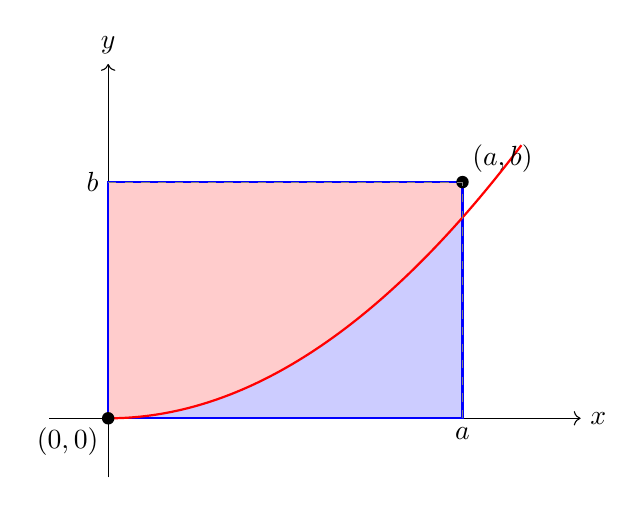
\begin{tikzpicture}[scale=1.5]
        % Draw axes
        \draw[->] (-0.5,0) -- (4,0) node[right] {$x$};
        \draw[->] (0,-0.5) -- (0,3) node[above] {$y$};
        
        % Define a and b
        \def\a{3}
        \def\b{2}
        
        % Shade area below the curve
        \fill[blue!20] (0,0) -- plot[domain=0:\a, samples=100] (\x, {1.7*(\x/\a)^2}) -- (\a,0) -- cycle;
        
        % Shade area above the curve
        \fill[red!20] plot[domain=0:\a, samples=100] (\x, {1.7*(\x/\a)^2}) -- (\a,\b) -- (0,\b) -- (0,0);
        
        % Draw rectangle
        \draw[blue, thick] (0,0) rectangle (\a,\b);
        
        % Draw exponential function extended beyond (a,b)
        \draw[red, thick, domain=0:3.5, samples=100] plot (\x, {1.7*(\x/\a)^2});
        
        % Label vertices
        \node[below left] at (0,0) {$(0,0)$};
        \node[above right] at (\a,\b) {$(a,b)$};
        
        % Mark points
        \fill (0,0) circle (1.5pt);
        \fill (\a,\b) circle (1.5pt);
        
        % Draw dashed lines to axes
        \draw[dashed, gray] (\a,0) -- (\a,\b);
        \draw[dashed, gray] (0,\b) -- (\a,\b);
        
        % Label axes values
        \node[below] at (\a,0) {$a$};
        \node[left] at (0,\b) {$b$};
      \end{tikzpicture}
      \caption{Rectangle with exponentially increasing curve and shaded regions}
      \label{fig:rectangle}
    \end{figure}

    We can see that the blue region has area 
    \begin{equation}
      \int_0^a x^{p-1} \,dx = \frac{a^p}{p} 
    \end{equation}
    We see that the red region has area $A$, 
    \begin{equation}
      A \leq \int_0^b y^{\frac{1}{p-1}} \,dy = \frac{y^{\frac{1}{p-1} + 1}}{\frac{1}{p-1} + 1} \bigg|_0^b = \frac{b^q}{q} 
    \end{equation}
  \end{proof}

  \begin{theorem}[Holder]
    Let $E$ be measurable, $1 \leq p \leq \infty$, $q = \frac{p}{p-1}$. Suppose $f \in L^p, g \in L^q$. Then, $f, g \in L^1 (E)$, and 
    \begin{equation}
      \int_E |fg| \,dx \leq \|f\|_p \|g\|_q
    \end{equation}
    In fact, this is sharp. If $f \neq 0$, then (note that this is the dual vector of $f$)
    \begin{equation}
      f^\ast (x) \coloneqq \|f\|_p^{1 - p} \mathrm{sgn}(f(x)) |f(x)|^{p-1} \in L^q
    \end{equation}
    with 
    \begin{equation}
      \|f^\ast \|_q = 1, \quad \int f f^\ast \,dx = \|f\|_p
    \end{equation}
  \end{theorem}
  \begin{proof}
    If $p =1$ ,or $p = \infty$, then this can be proven by monotonicity. If $1 < p < \infty$, then assume that $\|f\|_p = \|g\|_q = 1$, since by linearity, we can just normalize them by multiplying them by a constant. Not it suffices to prove that the integral $\leq 1$. Then, by Young's inequality,
    \begin{equation}
      |f(x) g(x)| \leq \frac{|f(x)|^p}{p} + \frac{|g(x)|^q}{q}
    \end{equation}
    and by integrating over $E$, since the RHS is integrable (it is also bounded?), we get 
    \begin{equation}
      \int_E |f(x) g(x)| \,dx \leq \frac{1}{p} + \frac{1}{q} = 1
    \end{equation}

    Finally, 
    \begin{equation}
      \|f^\ast\|_q^q = \|f\|_p^{(1-p) q} \int |f(x)|^{(p-1)q} \,dx = \|f\|_p^{-p} \int |f(x)|^p \,dx = 1
    \end{equation}
  \end{proof}

  \begin{corollary}[Cauchy-Schwartz]
    If $p = q = 2$, then we get Cauchy Schwartz. 
  \end{corollary}

  \begin{theorem}[Minkowski]
    If $f, g \in L^p$, then $f + g \in L^p$, and we get 
    \begin{equation}
      \| f + g \|_p \leq \|f\|_p + \|g\|_q
    \end{equation}
    This is the third condition for a norm. For $p = 1, +\infty$, this is immediate. Given $h \in L^p$, define 
    \begin{equation}
      h^\ast \coloneqq \|f\|_p^{1-p} \mathrm{sgn}(h) \, |h|^{p-1} 
    \end{equation}
    Then, from the previous theorem, 
    \begin{align}
      \| f + g \|_p & = \int_E (f + g)(f + g)^\ast \,dx  \\ 
                    & = \int_E f (f + g)^\ast \,dx + \int_E g (f + g)^\ast \,dx  \\ 
                    & \leq \|f\|_p \underbrace{\|(f + g)^\ast\|_q}_{1} + \|g\|_p \underbrace{\|(f + g)^\ast\|_q}_{1} 
    \end{align}
  \end{theorem}

  The following is an easy way to check that $\mathscr{F}$ is equi-integrable. 

  \begin{corollary}
    let $\mathscr{F}$ be a family of functions s.t. 
    \begin{equation}
      \int |f|^p \,dx < +\infty \forall f \in \mathscr{F}
    \end{equation}
    Then $\mathscr{F}$ is equi-integrable. 
  \end{corollary}
  \begin{proof}
    Let $A$ be ameasurable, $m(A) \leq \delta$. Then 
    \begin{equation}
      \int_A |f| \,dx \leq \bigg( \int_A |f|^p \bigg)^{1/p} \bigg( \int_A 1^q \bigg)^{1/q} \leq M^{1/p} m(A) \leq m^{1/p} \delta^{1/q} 
    \end{equation}
    Given any $\epsilon > 0$, we can choose $\delta > 0$ s.t. $\int |f| \,dx \leq \epsilon$ if $m(A) < \delta$. 
  \end{proof}

  \begin{corollary}
    Assume $E$ has finite measure. Then, $L^{p_1} \subset L^{p_2}$ for any $1 \leq p_1 \leq p_2 \leq +\infty$. So a higher exponent is more restrictive in a finite measure set. 
  \end{corollary}
  \begin{proof}
    A simple application of Holder's inequality. 
    \begin{equation}
      \int_E |f|^{p_1} \leq \bigg( \int_E |f|^{p_2} \,dx \bigg)^{p_1/p_2} x 
    \end{equation}
  \end{proof}

  In infinite measures, there are two ways that this can fail: singularities or tails. Either because it blows up, or it doesn't decay fast enough to be in $L^p$. $x^{-\alpha}$. 

\subsection{Nov 3} 

  \begin{example}
    Consider $f_m (x)$ in $L^p [0, 1]$, with 
    \begin{equation}
      f_m (x) =  \chi_{I_k^{(n)}} (x) \cdot 2^{n/p}, \quad I_k^{(n)} = [ (k-1) 2^{-n}, k 2^{-n}] 
    \end{equation}
    Note that $\|f_m\|_{L^p} = 1$, but $\|f_{m_1} - f_{m_2}\|_{L^p} \geq \frac{1}{2}$. So there are no limit points in $f_m$. 
  \end{example}

  \begin{definition}[Dual Vector]
    Suppose $X$ is a Banach space. Then $\mathcal{L}: X \to \mathbb{R}$ is called a \textbf{linear bounded functional} on $X$ if 
    \begin{equation}
      \mathcal{L}(\alpha f + \beta g)  = \alpha \mathcal{L} f + \beta \mathcal{L} g, \quad \forall f, g \in X
    \end{equation}
    and  
    \begin{equation}
      | \mathcal{L} (f)| \leq \|\mathcal{L}\|_\ast \|f\|, \quad \forall f \in X
    \end{equation}
  \end{definition}

  Whenever you want to prove that an integral is bounded, then you use Holder. 

  \begin{example}
    Let $X = L^p (E)$. Then 
    \begin{equation}
      \mathcal{L} f \coloneqq \int f g \,dx, \quad g \in L^q, q = \frac{p}{p - 1}
    \end{equation}
    is a linear bounded functional (by Holder). 
  \end{example}

  $L^\infty$ is not separable (as in there is no dense countable subset). 

  \begin{theorem}
    Given a Banach space $X$, the space of all linear bounded functionals on $X$ is a linear space with norm 
    \begin{equation}
      \|\mathcal{L}\|_\ast = \sup_{f \in X, \|f\| \leq 1} | \mathcal{L} (f) |
    \end{equation}
    This space is called \textbf{dual} to $X$, denoted $X^\ast$. 
  \end{theorem}
  \begin{proof}
    Just check that the sum, scalar multiplication is still a linear functional. Then for norm, just use triangle inequality. 
  \end{proof}

  We would like to prove that $(L^p)^\ast = L^q$, which we will do later. Now we'll define a different form of convergence. The regular pointwise convergence is known as strong convergence. 

  \begin{definition}[Weak Convergence]
    We say $f_n \rightharpoonup f$, i.e. \textbf{converges weakly} on $X$ if 
    \begin{equation}
      \mathcal{L}(f_n) \to \mathcal{L}(f), \quad \forall \mathcal{L} \in X^\ast
    \end{equation}
  \end{definition}


  \begin{example}
    Let $f_m(x)$ as before, and fix $g \in L^q [0, 1]$. Then, by Holder, 
    \begin{equation}
      \bigg| \int_0^1 \chi_{I_k^{(n)}} (x) g(x)\,dx  \bigg| \leq \|f_m\|_{L^p} \cdot \| g \cdot \chi_{I_k^{(n)}}\|_{L^q} \to 0, \text{ as } m \to +\infty
    \end{equation}
    since 
    \begin{equation}
      \int_{I_k^{(n)}} |g|^p \,dx \to 0 \text{ as } n \to +\infty
    \end{equation}
    by DCT, since $I_k^{(n)} = [(k-1) 2^{-n}, k 2^{-n}]$. 
  \end{example}

  So if we know that $(L^p)^\ast = L^q$, we could conclude $f_m \rightharpoonup 0$. 

  \begin{lemma}
    Suppose $\mathcal{L}_1, \mathcal{L}_2 \in X^\ast$. Suppose $Y$ is a dense subset of $X$. If $\mathcal{L}_1 = \mathcal{L}_2$ on $Y$, then $\mathcal{L}_1 = \mathcal{L}_2$. 
  \end{lemma}
  \begin{proof}
    Take any $g \in X$. Find $f \in Y$ s.t. $\|f - g\|_X \leq \epsilon$. Then, 
    \begin{align}
      |\mathcal{L}_1 g - \mathcal{L}_2 g| 
        & \leq |\mathcal{L}_1 g - \mathcal{L}_1 f| + \underbrace{|\mathcal{L}_1 f - \mathcal{L}_2 f|}_{=0} + |\mathcal{L}_2 f - \mathcal{L}_2 g| \\ 
        & \leq (\|\mathcal{L}_1\|_\ast + \| \mathcal{L}_2\|_\ast) \epsilon
    \end{align}
  \end{proof}

  \begin{lemma} 
    Let $E \subset \mathbb{R}$ be measurable, $1 \leq p \leq +\infty$. Suppose $g \in L^1 (E)$ and 
    \begin{equation}
      \bigg| \int_E f g \,dx \bigg| \leq M \| f\|_p, \quad \forall f \in L^p \text{ simple}
    \end{equation}
    Then, $g \in L^q, \|g\|_q \leq M$. 
  \end{lemma}
  \begin{proof}
    Consider $+\infty > p > 1$. Consider a sequence of simple $\varphi_n$ s.t. $\varphi_n \to |g|$ a.e., with $0 \leq \varphi_n \leq |g|$. Then, it suffices to show that 
    \begin{equation}
      \int | \varphi_n|^q \,dx \leq M, \quad \forall n
    \end{equation}
    since we can just invoke Fatou's lemma. Define simple $f_n = \mathrm{sgn}(g) |\varphi_n|^{q-1}$. Note $f_n \in L^p$ (simple functions). Then 
    \begin{equation}
      \int_E |\varphi_n|^q\,dx \leq  \int_E g \cdot f_n \,dx \leq M \|f_n \|_p, 
    \end{equation}
    where 
    \begin{equation}
      \|f_n\|_p = \bigg( \int | \varphi_n|^{q-1)p} \,dx \bigg)^{1/p} = \| \varphi_n \|_q^{q/p} 
    \end{equation}
    So $\| \varphi_n \|_q^{q- \frac{q}{p}} = \|\varphi_n\|_q \leq M$. Since $q(1 - \frac{1}{p}) = q \frac{1}{q} = 1$. 
  \end{proof}

  \begin{theorem}
    Let $[a, b]$ be a finite interval, with $1 \leq p < +\infty$. Suppose $\mathcal{L}$ is a linear bounded functional on $L^p([a, b])$. Then $\exists g \in L^q ([a, b])$ s.t. $\mathcal{L}f = \int_a^b f g \,dx$. 
  \end{theorem}
  \begin{proof}
    Suppose $p > 1$. Define $\phi(x) = \mathcal{L}(\chi_{[0, x]})$. We claim that $\phi$ is AC. Take $[a_k, b_k]_{k=1}^n$ disjoint in $[a, b]$. We have 
    \begin{equation}
      \sum_{k=1}^n |\phi(b_k) - \phi(a_k)|
    \end{equation}
    Given $\epsilon > 0$, we want to show that $\exists \delta >0$ s.t. 
    \begin{equation}
      \sum_{k=1}^n |b_k - a_k| \leq \delta \implies \sum_{k=1}^n |\phi(b_k) - \phi(a_k)| < \epsilon 
    \end{equation}
    But 
    \begin{align}
      \sum_{k=1}^n |\phi(b_k) - \phi(a_k)| & = \mathcal{L} \underbrace{\bigg( \sum_{k=1}^n \mathrm{sgn} \big( \phi(b_k) - \phi(a_k) \big) \chi_{[a_k, b_k]} \bigg)}_{f} \\ 
      & \leq \|\mathcal{L}\|_\ast \|f\|_p \\ 
      & = \|\mathcal{L}\|_\ast \bigg( \sum_{k=1}^n (b_k - a_k) \bigg)^{1/p}
    \end{align}
    Take $\delta = \big( \frac{\epsilon}{\|\mathcal{L}\|_\ast} \big)^{p}$
  \end{proof}

  So now that we have proved that $\phi$ is AC, we are almost in a position to use the lemma we proved before. Then, $\exists g \in L^1$ s.t. $\phi(x) = \int_a^x g(t) \,dt$ by fundamental theorem of calculus. Given ay $\chi_{[c, d]}$, we have 
  \begin{equation}
    \mathcal{L}(\chi_{c, d}) = \phi(d) - \phi(c) = \int_c^d g(t) \,dtjjA
  \end{equation}
  So $\mathcal{L} f$ and $\int g f \,dx$ coincide on step functions, and step functions are a dense set in $L^p$. We have 
  \begin{equation}
    \bigg| \int g f \,dx \bigg| \leq \|\mathcal{L}\|_\ast \|f\|_p 
  \end{equation}
  By the lemma, $g \in L^q$, with $\|g\|_q \leq \|\mathcal{L}\|_\ast$. 

  Note that this is \textit{not true} on $L^\infty$. Indeed $(L^1)^\ast = L^\infty$ (this is easier to prove), but $(L^\infty)^\ast \neq L^1$. But it is hard to construct a counterexample, and people use the Banach extension theorem to define such counterexamples. 

  \begin{theorem}[Riesz Representation Theorem]
    Let $E \subset \mathbb{R}$ be measurable, $1 \leq p < +\infty$. Suppose $\mathcal{L}$ is a bounded linear functional on $L^p$. Then $\exists g \in L^q$ s.t. 
    \begin{equation}
      \mathcal{L}(f) = \int_E g f \,dx, \quad \|g\|_q = \|\mathcal{L}\|_\ast
    \end{equation}
  \end{theorem}

  The dual of continuous functions is Steljes measures. 

  Now let's talk about weak convergence. This gives you some sort of compactness of a unit ball in $X^\ast$ with respect to the norm, which is basically sort of like weak convergence. 

  \begin{theorem}[Helley]
    Lt $X$ be a Banach space, separable. Suppose $\mathcal{L}_n \in X^\ast$ satisfy $\|L_n\|_\ast \leq M$ for all $n$. Then, $\exists n_k$ s.t. 
    \begin{equation}
      L_{n_k} (f) \to L (f), \quad \forall f \in X
    \end{equation}
  \end{theorem}
  \begin{proof}
    Let $(f_n)_{n=1}^\infty$ be a countable dense subset in $X$. Then, $\{\mathcal{L}_n f_1\}_{n=1}^\infty$ is ? $\implies \exists$ subsequence $s_{1, m}$ s.t. $\mathcal{L}_{s_{1, m}} f_1 \to a_1$. Also, we can choose a $s_{2, m}$ subsequence of $s_{1, m}$ s.t. $\mathcal{L}_{s_2, m} f_2 \to a_2$, and so in $s_{l, m}$ s.t. 
    \begin{equation}
      \mathcal{L}_{s_{l, m}} f_j \to a_j, \quad \forall 1 \leq j \leq l
    \end{equation}
    Select $n_k = S_{k, k}$. Then, $\mathcal{L}_{n_k} f_j \to a_j$ for all $j$. Given any $g \in X$, consider 
    \begin{equation}
      |\mathcal{L}_{n_{k_2}} g - \mathcal{L}_{n_{k_1}} g| \leq |\mathcal{L}_{n_{k_2}} g - \mathcal{L}_{n_{k_1}} f| + |\mathcal{L}_{n_{k_2}} f - \mathcal{L}_{n_{k_1}} f| + |\mathcal{L}_{n_{k_2}} f - \mathcal{L}_{n_{k_1}} g|
    \end{equation}
    Fix $\epsilon > 0$, choose $f$ s.t. 
    \begin{equation}
      \|f - g\| \leq \frac{\epsilon}{3 \max\{\|f\|, \|g\|\}}
    \end{equation}
    Then, $k_1, k_2$, large so middle term $\leq \frac{\epsilon}{3}$. 
  \end{proof}

  So this is what people mean by a unit ball in $L^p$ is weakly compact. 

\subsection{Exercises} 

  \begin{exercise}[Math 631 Fall 2025, Final Exam Exercise 6]
    Define $c_{0}$ to be a space of all sequences $x=x_{1},x_{2},...,x_{n},...$ that converge to zero, with the norm $\|x\|=\sup_{n}|x_{n}|$. Prove that $c_{0}$ is a Banach space and find its dual.
  \end{exercise}
  \begin{solution}
    Suppose that $x^{m}$ is a Cauchy sequence in $c_{0}$. Then each component $x_{n}^{m}$ is also a Cauchy sequence of real numbers, and converges to some $y_{n}$. It is not hard to see that $y_{n}$ is a bounded sequence: take $\epsilon=1$ and find $N$ such that $\|x^{m}-x^{N}\|_{\infty}\le1$ if $m\ge N$. Then also $\|y-x^{N}\|_{\infty}\le1$, and so $y\in l^{\infty}$. Let us now show that $y\in c_{0}$. Fix $\epsilon>0$. Find $N$ such that $\|y-x^{N}\|_{\infty}\le\epsilon/2$. Next, since $x^{N}\in c_{0}$, find $M$ such that $|x_{m}^{N}|\le\epsilon/2$ for all $m\ge M$. Then for every $m\ge M$,
    \begin{equation}
      |y_{m}|\le|y_{m}-x_{m}^{N}|+|x_{m}^{N}|\le\epsilon.
    \end{equation}
    Hence $y\in c_{0}$. This proves $c_{0}$ is a Banach space.

    Take any sequence $a_{n}$ in $l_{1}$, then it defines a bounded linear functional $A$ on $c_{0}$ defined by $A(x)=\sum_{n=1}^{\infty}a_{n}x_{n}$. Note that $\|A\|=\|a\|_{l^{1}}$: we can just take sequences $x_{n}^{m}$ that take value 1 if $a_{n}>0$ and -1 if $a_{n}<0$ for $n=1,...,m$. Then $\|x^{m}\|_{\infty}=1$, and
    \begin{equation}
      \sum_{n=1}^{\infty}a_{n}x_{n}^{m}\rightarrow\|a\|_{l^{1}}
    \end{equation}
    as $m\rightarrow\infty$ by Lebesgue dominated convergence theorem. On the other hand, let $A$ be any bounded linear functional on $c_{0}$. For every $n$, take $e^{n}\in c_{0}$ such that $e_{j}^{n}=\delta_{nj}$ (1 if $j=n$ and 0 if $j\ne n$). Set $a_{n}=A(e_{n})$. By taking $x^{m}$ before equal to $\pm1$ depending on the sign of $a_{n}$ for the first $m$ positions, we find that
    \begin{equation}
      A(x^{m})=\sum_{n=1}^{m}|a_{n}|\le\|A\|,
    \end{equation}
    for every $m$. Therefore, $a_{n}\in l^{1}$ and then it is not hard to see $\|A\|=\|a\|_{l^{1}}$. Hence the dual space of $c_{0}$ can be identified with $l^{1}$.
  \end{solution}

  \begin{exercise}[Math 631 Fall 2025, Final Exam Exercise 7]
    Let $h$ be continuous function periodic on $\mathbb{R}$ with period one, and assume $\int_{0}^{1}h(x)dx=0$. Define $f_{n}(x)=h(nx)$. Show that for any finite interval $[a, b]$, $f_{n}\rightarrow0$ in $L^{p}[a,b]$, $1\le p<\infty$.
  \end{exercise}
  \begin{solution}
    Since step functions are dense in $L^{p}[a,b]$, it suffices to prove that for any $a\le c < d\le b,$ $\int_{c}^{d}h(nx)dx\rightarrow0$ as $n\rightarrow\infty$. But
    \begin{equation}
      \int_{c}^{d}h(nx)dx=n^{-1}\int_{nc}^{nd}h(y)dy\le2\|h\|_{L^{\infty}}n^{-1}\rightarrow0
    \end{equation}
    as $n\rightarrow\infty$. Here we used that periodic continuous function must be bounded, and integrated over all full periods included into $[nc, nd]$ getting zero from these parts since $h$ is mean zero.
  \end{solution}


\section{Measure}

  Now we generalize to abstract measure spaces. Recall how we constructed the Lebesgue measure: (1) We took a set function $\ell$ that assigns lengths to all intervals in $\mathbb{R}$. (2) We have used this length to define the Lebesgue outer measure as an outer approximation of these intervals. (3) We then use the outer measure to define measurable sets with Caratheodory's criterion, which states that measurable sets should split any set nicely into measurable sets. (4) We verify that the collection of all measurable sets is a $\sigma$-algebra. (5) We define the Lebesgue measure as the restriction of the Lebesgue outer measure to the collection of mesaurable sets. This is called the \textit{Caratheodory} construction of Lebesgue measure, and we can generalize this to an abstract space $X$ under certain conditions.  

  First, we want all measurable sets to be a $\sigma$-algebra, which defines all the well-behaved sets. 

  \begin{definition}[Measurable Space] 
    A \textbf{measurable space} is a tuple $(X, \mathcal{M})$ consisting of a set $X$ with a $\sigma$-algebra of subsets of $X$. Elements of $\mathcal{M}$ are called \textbf{measurable sets}. 
  \end{definition}

  \begin{definition}[Measure, Measure Space]
    A \textbf{measure} $\mu$ on a measurable space $(X, \mathcal{M})$ is a set function $\mu: \mathcal{M} \to [0, +\infty]$ satisfying the following. 
    \begin{enumerate}
      \item \textit{Null empty set}. $\mu(\emptyset) = 0$. 
      \item \textit{Countable Additivity}. For all countable collections $\{A_k\}_{k=1}^\infty$ of pairwise disjoint\footnote{Disjointness is clearly important since if it wasn't, then $\mu(A) = \mu(A \cup A) = 2 \mu(A)$, which is absurd. } subsets $A_k \subset 2^{X}$,
      \begin{equation}
        \mu \bigg( \bigsqcup_{k=1}^\infty A_k \bigg) = \sum_{k=1}^\infty \mu(A_k)
      \end{equation}
    \end{enumerate} 
  \end{definition}

  \begin{example}[Measure Spaces]
    The following are all valid measure spaces. 
    \begin{enumerate}
      \item $(\mathbb{R}, \mathcal{L}, m)$, where $\mathcal{L}$ is the set of all Lebesgue-measurable sets. 
      \item $(\mathbb{R}, \mathcal{B}, m)$, where $\mathcal{B}$ is the set of all Borel-measurable sets. 
      \item $(X, 2^X, \eta)$, where $\eta(E)$ is the cardinality of the set. This is called the \textbf{counting measure}. 
      \item $(X, 2^X, \delta_{x_0})$ where $x_0 \in X$ and $\delta_{x_0}(E) = 1$ if $x_0 \in E$ and $0$ if else. This is called the \textbf{Dirac measure}. 
    \end{enumerate}
  \end{example}

  From just this definition, we can restore all of our familiar properties. 

  \begin{theorem}[Axiomatic Properties of Measure]
    Let $(X, \mathcal{M}, \mu)$ be a measure space. 
    \begin{enumerate}
      \item \textit{Finite Additivity}. For any finite disjoint collection $\{E_k\}_{k=1}^n$ of measurable sets, 
        \begin{equation}
          \mu \bigg( \bigcup_{k=1}^n E_k \bigg) = \sum_{k=1}^n \mu(E_k)
        \end{equation}
      \item \textit{Monotonicity}. If $A \subset B$ are both measurable sets, then 
        \begin{equation}
          \mu(A) \leq \mu(B)
        \end{equation}
      \item \textit{Excision}. If $A \subset B$ are both measurable sets and $\mu(A) < +\infty$, then 
        \begin{equation}
          \mu(B \setminus A) = \mu(B) - \mu(A)
        \end{equation}
      \item \textit{Countable Monotonicity}. For any countable collection $\{E_k\}_{k=1}^\infty$ of measurable sets that covers a measurable set $E$, 
        \begin{equation}
          \mu(E) \leq \sum_{k=1}^\infty \mu(E_k)
        \end{equation}
    \end{enumerate}
  \end{theorem}
  \begin{proof}
    Listed. 
    \begin{enumerate}
      \item \textit{Finite Additivity}. 
      \item \textit{Monotonicity}. Let $B \setminus A \coloneqq B \cap A^c$. Then, since $A$ and $B \setminus A$ are disjoint, we have 
        \begin{equation}
          \mu(B) = \mu\big( A \cup (B \setminus A) \big) = \mu(A) + \mu(B \setminus A) \geq \mu(A)
        \end{equation}

      \item \textit{Excision}.
      \item \textit{Countable Monotonicity}. We again try to divide this union into disjoint sets. Let $A_i^\prime = A \cap A_i$, and let $B_1 = A_1^\prime$ with 
        \begin{equation}
          B_i = A_i \setminus \bigcup_{j=1}^{i-1} A^\prime_j
        \end{equation}
        Since $B_i$'s are disjoint with $B_i \subset A_i$, we can use the first property to get 
        \begin{equation}
          \mu(A) = \sum_{i=1}^\infty \mu(B_i) \leq \sum_{i=1}^\infty \mu(A_i)
        \end{equation}

    \end{enumerate}
  \end{proof}

  \begin{theorem}[Continuity of Measure]
    Let $(X, \mathcal{M}, \mu)$ be a measure space. 
    \begin{enumerate}
      \item \textit{Continuity from Below}. If $\{A_k\}_{k=1}^\infty$ is an ascending sequence of measurable sets, then 
        \begin{equation}
          \mu \bigg( \bigcup_{k=1}^\infty A_k \bigg) = \lim_{k \to \infty} A_k
        \end{equation}
      \item \textit{Continuity from Above}. If $\{B_k\}_{k=1}^\infty$ is a descending sequence of measurable sets and $\mu(B_1) < +\infty$, then 
        \begin{equation}
          \mu \bigg( \bigcap_{k=1}^\infty B_k \bigg) = \lim_{k \to \infty} \mu(B_k)
        \end{equation}
    \end{enumerate}
  \end{theorem}
  \begin{proof}
    Listeed. 
    \begin{enumerate}
      \item \textit{Continuity from Below}. With the fact that $\mu(A_k)$ must be nondecreasing, we can use real analysis and see that it is bounded by $\infty$, meaning that it must have a limit. But why does this limit equal to the left hand side? We can see that 
        \begin{align}
          \mu\bigg( \bigcup_{k=1}^\infty A_k \bigg) & = \mu(A_1) + \sum_{k=2}^\infty \mu(B_k) \\
          & = \mu(A_1) + \lim_{k \rightarrow \infty} \sum_{k=2}^\infty \mu(B_k) \\
          & = \lim_{k \rightarrow \infty} \mu(A_1 \cup B_2 \cup \ldots B_k)  = \lim_{k \rightarrow \infty} \mu(A_k) 
        \end{align}
        where $B_k = A_k \setminus A_{k-1}$. 

      \item \textit{Continuity from Above}. The $\mu(A_1) < \infty$ is a necessary condition, since if we take $A_k = [k, \infty)$ on the real number line, then we have $\cap_{k=1}^\infty A_k = \emptyset$, but the limit of the measure is $\infty$. Well we can define $B_k = A_k \setminus A_{k+1}$ and write $\cap_{k=1}^\infty A_k = A_1 \setminus \cup_{k=1}^\infty B_k$, which means that 
        \begin{align}
          \mu\bigg( \bigcap_{k=1}^\infty A_k \bigg) & = \mu\bigg( A_1 \setminus \bigcup_{k=1}^\infty B_k \bigg) \\
          & = \mu(A_1) - \mu\bigg( \bigcup_{k=1}^\infty B_k\bigg) \\
          & = \mu(A_1) - \sum_{k=1}^\infty \mu(B_k) \\
          & = \mu(A_1) - \lim_{K \rightarrow \infty} \sum_{k=1}^K \mu(B_k) \\
          & = \lim_{K \rightarrow \infty} \bigg( \mu(A_1) - \sum_{k=1}^K \mu(B_k) \bigg) \\
          & = \lim_{K \rightarrow \infty} \mu \bigg( A_1 \setminus \bigcup_{k=1}^K B_k \bigg) = \lim_{K \rightarrow \infty} \mu(A_K)
        \end{align}
        Now the first line uses the fact that if $A \subset B$, then $\mu(B \setminus A) + \mu(A) = \mu(B)$, and with the further assumption that $\mu(A) < \infty$, we can subtract on both sides like we do with regular arithmetic. 
    \end{enumerate}
  \end{proof}

  \begin{definition}[Almost Everywhere]
    For a measure space $(X, \mathcal{M}, \mu)$ and a measurable subset $E$ of $X$, we say that a property $P$ holds \textbf{almost everywhere} on $E$ if it holds for all $E \setminus E_0$ for some measurable subset $E_0$ where $\mu(E_0) = 0$.
  \end{definition}

  \begin{lemma}[Borel-Cantelli Lemma]
    Let $(X, \mathcal{M}, \mu)$ be a measure space and $\{E_k\}_{k=1}^\infty$ be a countable collection of measurable sets for which $\sum_{k=1}^\infty \mu(E_k) < +\infty$. Then, 
    \begin{equation}
      \mu \big( \limsup_k E_k \big) \coloneqq \mu \bigg( \bigcap_{n = 1}^\infty \bigcup_{k \geq n} E_k \bigg) = 0
    \end{equation}
    That is, almost all $x \in X$ belong to at most a finite number of the $E_k$'s. 
  \end{lemma}
  \begin{proof}
    By continuity of $\mu$ from above and countable monotonicity of $\mu$, 
    \begin{equation}
      \mu \bigg( \bigcup_{n=1}^\infty \bigg[ \bigcap_{k \geq n} E_k \bigg] \bigg) = \lim_{n \to \infty} \mu \bigg( \bigcup_{k \geq n} E_k \bigg) \leq \lim_{n \to\infty} \sum_{k = n}^\infty \mu(E_k) = 0
    \end{equation}
    since the series converges. 
  \end{proof}

  Now here comes the new part. 

  \begin{definition}[Finite, $\sigma$-Finite Measures and Measurable Sets]
    Let $(X, \mathcal{M}, \mu)$ be a measure space. 
    \begin{enumerate}
      \item The measure $\mu$ is \textbf{finite} if $\mu(X) < +\infty$. 
      \item The measure $\mu$ is \textbf{$\sigma$-finite} if $X$ is the union of a countable collection of measurable sets, each of which has finite measure. 
    \end{enumerate}
    Let $E$ be a measurable set. 
    \begin{enumerate}
      \item $E$ is of \textbf{finite measure} if $\mu(E) < +\infty$. 
      \item $E$ is \textbf{$\sigma$-finite} if $E$ is the union of a countable collection of measurable sets, each of which has finite measure. 
    \end{enumerate}
    Finiteness implies $\sigma$-finiteness. 
  \end{definition}

  \begin{example}
    Listed. 
    \begin{enumerate}
      \item The Lebesgue measure on $[0, 1]$ is a finite measure. 
      \item The Lebesgue measure on $\mathbb{R}$ is a $\sigma$-finite measure. 
      \item The counting measure on an uncountable set is not $\sigma$-finite.  
    \end{enumerate}
  \end{example}

  \begin{definition}[Complete Metric Spaces]
    A measure space $(X, \mathcal{M}, \mu)$ is \textbf{complete} if $\mathcal{M}$ contains all subsets of sets of measure $0$. 
  \end{definition}

  \begin{example}
    Listed. 
    \begin{enumerate}
      \item $(\mathbb{R}, \mathcal{L}, m)$ is complete. 
      \item $(\mathbb{R}, \mathcal{B}, m)$ is complete since we shows that the Cantor set (a Borel set of Lebesgue measure $0$), contains a subset that is not Borel. 
    \end{enumerate}
  \end{example}

  \begin{theorem}[Every Measure Space can be Completed]
    Let $(X, \mathcal{M}, \mu)$ be a measure space. Define $\mathcal{M}_0$ to be the collection of subsets $E$ of $X$ of the form $E = A \cup B$ where 
    \begin{enumerate}
      \item $B \in \mathcal{M}$, 
      \item $A \subset C$ for some $C \in \mathcal{M}$ for which $\mu(C) = 0$.\footnote{So we are basically splitting $E$ into a measure $0$ part $C$ and everything else $B$.}
    \end{enumerate}
    For such a set $E$, define $\mu_0 (E) = \mu(B)$. Then, $\mathcal{M}_0$ is a $\sigma$-algebra that contains $\mathcal{M}$, $\mu_0$ is a measure that extends $\mu$, and $(X, \mathcal{M}_0, \mu_0)$ is a complete measure space. 
  \end{theorem}
  \begin{proof}
    
  \end{proof}

\subsection{Signed Measures}

  \begin{lemma}[Sums and Positive Multiples of Measures are Measures]
    If $\mu_1$ and $\mu_2$ are two measures defined on the same measurable space $(X, \mathcal{M})$, then for $\alpha, \beta > 0$, the following is a measure as well. 
    \begin{equation}
      \mu_3 (E) = \alpha \cdot \mu_1 (E) + \beta \cdot \mu_2 (E)
    \end{equation}
  \end{lemma}
  \begin{proof}
    
  \end{proof}

  Note that we can't always define differences of such measures 
  \begin{equation}
    \nu(E) = \mu_1 (E) - \mu_2 (E)
  \end{equation}
  since $\nu$ may not always be nonnegative. Furthermore, it may not even be defined if $\mu_1 (E) - \mu_2 (E) = \infty - \infty$. 

  \begin{definition}[Signed Measure]
    A \textbf{signed measure} $\nu$ on the measurable space $(X, \mathcal{M})$ is a function $\nu: \mathcal{M} \to [-\infty, +\infty]$ satisfying 
    \begin{enumerate}
      \item \textit{Well-Defined}. $\nu$ assumes at most one of the values $+\infty, -\infty$. 
      \item \textit{Null Empty Set}. $\nu(\emptyset) = 0$ 
      \item \textit{Countable Additivity}. For any countable collection $\{E_k\}_{k=1}^\infty$ of disjoint measurable sets, 
        \begin{equation}
          \nu \bigg( \bigcup_{k=1}^\infty E_k \bigg) = \sum_{k=1}^\infty \nu(E_k)
        \end{equation}
        where the series $\sum_{k} \nu(E_k)$ converges absolutely if $\nu \big( \cup_{k} E_k \big)$ is finite. 
    \end{enumerate}
  \end{definition} 

  \begin{definition}[Positive, Negative, Null Sets]
    Let $\nu$ be a signed measure on $(X, \mathcal{M})$ and $A \in \mathcal{M}$. 
    \begin{enumerate}
      \item $A$ is \textbf{positive} w.r.t. $\nu$ if for all measurable $E \subset A$, $\nu(E) \geq 0$. 
      \item $A$ is \textbf{negative} w.r.t. $\nu$ if for all measurable $E \subset B$, $\nu(E) \leq 0$. 
      \item $A$ is \textbf{null} w.r.t. $\nu$ if for all measurable $E \subset B$, $\nu(E) = 0$.\footnote{By monotoncity of measure, a set is null if and only if it has measure $0$.}
    \end{enumerate}
  \end{definition}

  \begin{lemma}[Hahn's Lemma]
    Let $\nu$ be a signed measure on $(X, \mathcal{M})$ and $E$ a measurable set for which $0 < \nu(E) < +\infty$. Then, there is a measurable subset $A \subset E$ that is positive and of positive measure. 
  \end{lemma}

  \begin{theorem}[Hahn Decomposition Theorem]
    Let $\nu$ be a signed measure on the measurable space $(X, \mathcal{M})$. Then, there is a positive set $A$ and a negative set $B$, both with respect to $\nu$, for which 
    \begin{equation}
      X = A \sqcup B
    \end{equation}
    That is, we can always decompose $X$ into a positive and negative measure parts, and this is called the \textbf{Hahn decomposition} of $X$ w.r.t. $\nu$.\footnote{Note that this may not be unique, since if $A \cup B$ is a Hahn decomposition, then by excising a null set $E$ from $A$ and adding to $B$, $(A \setminus E) \cup (B \cup E)$ is also a Hahn decomposition.} 
  \end{theorem}

  Therefore, the measure of $\nu^+ (E) = \nu (E \cap A)$ and $\nu^- (E) = -\nu(E \cap B)$. This decomposition is nice since we know that the positive parts and the negative parts are ``nicely separated.'' Let's formalize this notion. 

  \begin{definition}[Mutually Singular Measures]
    Two measures $\nu_1, \nu_2$ are said to be \textbf{mutually singular}, denoted $\nu_1 \perp \nu_2$, if $X = A \cup B$ with $\nu_1 (A) = \nu_2 (B) = 0$. 
  \end{definition}

  \begin{theorem}[Jordan Decomposition Theorem]
    Let $\nu$ be a signed measure on the measurable space $(X, \mathcal{M})$. Then, there is a unique pair of mutually singular measures $\nu^+, \nu^-$ on $(X, \mathcal{M})$ for which 
    \begin{equation}
      \nu = \nu^+ - \nu^- 
    \end{equation}
    called the \textbf{Jordan decomposition}, with $\nu^+, \nu^-$ called the positive and negative parts of $\nu$. Since $\nu$ assumes at most one of the values $\pm \infty$, either $\nu^+, \nu^-$ must be finite. 
  \end{theorem}
  \begin{proof}
    We have already proven the first part as 
    \begin{equation}
      \nu^+ (E) = \nu (E \cap A), \quad \nu^- (E) = -\nu(E \cap B)
    \end{equation}
  \end{proof}

  \begin{example}[]
    Let $f: \mathbb{R} \to \mathbb{R}$ be a function that is Lebesgue integrable over $\mathbb{R}$, and define 
    \begin{equation}
      \nu(E) \coloneqq \int_E f \,dm
    \end{equation}
    Then, from the countable additivity of integration, $\nu$ is a signed measure on the measurable space $(\mathbb{R}, \mathcal{L})$. Define 
    \begin{equation}
      A = \{x \in \mathbb{R} \mid f(x) \geq 0 \}, \quad B = \{x \in \mathbb{R} \mid f(x) < 0 \}
    \end{equation}
    and 
    \begin{equation}
      \nu^+ (E) = \int_{A \cap E} f \,dm, \quad \nu^- (E) = - \int_{B \cap E} f \,dm
    \end{equation}
    Then, $A, B$ is a Hahn decomposition of $\mathbb{R}$ w.r.t. the signed measure $\nu$. Moreover, $v = v^+ = v^-$ is a Jordan decomposition of $\nu$. 
  \end{example}

\subsection{Carathéodory Construction of Measurable Sets} 

  \begin{definition}[Outer Measure]
    Given a space $X$, an \textbf{outer measure} is a function $\mu^\ast : 2^X \to [0, +\infty]$ satisfying either the two properties. 
    \begin{enumerate}
      \item \textit{Null Empty Set}. $\mu^\ast(\emptyset) = 0$. 
      \item \textit{Countable Monotonicity}. For arbitrary subset $A, B_1, B_2, \ldots$, 
      \begin{equation}
        A \subset \bigcup_{k=1}^\infty B_k \implies \mu(A) \leq \sum_{k=1}^\infty \mu(B_k)
      \end{equation} 
    \end{enumerate}
  \end{definition}

  \begin{theorem}[Construction of Outer Measure]
    Let $\mathcal{S}$ be a collection of subsets in $X$ and $\mu: \mathcal{S} \to [0, +\infty]$ be a set functions. Define $\mu^\ast(\emptyset) = 0$ and 
    \begin{equation}
      \mu^\ast (E) \coloneqq \inf \bigg\{ \sum_{k=1}^\infty \mu(E_k) \colon E \subset \bigcup_k E_k \bigg\}
    \end{equation}
    where the infimum of an empty set is $+\infty$. Then, the set function $\mu^\ast : 2^X \to [0, +\infty]$ is an outer measure called the \textbf{outer measure induced by $\mu$}. 
  \end{theorem}
  \begin{proof}
    
  \end{proof}

  \begin{definition}[Carathéodory's criterion]
    Given outer measure $\mu^\ast$ on $X$, a set $E \subset X$  is called \textbf{$\mu^\ast$-measurable} if for every set $A \subset X$, 
    \begin{equation}
      \mu^\ast (A \cap E) + \mu^\ast (A \cap E^c) = m^\ast (A) 
    \end{equation}
  \end{definition} 

  \begin{theorem}[Measurable Sets is a $\sigma$-Algebra]
    Let $\mu^\ast$ be an outer measure on $2^X$. Then, the collection $\mathcal{M}$ of sets that are measurable w.r.t. $\mu^\ast$, also called $\mu^\ast$-measurable, is a $\sigma$-algebra. If $\overline{\mu}$ is the restriction of $\mu^\ast$ to $\mathcal{M}$, then $(X, \mathcal{M}, \overline{\mu})$ is a complete measure space. 
  \end{theorem}
  \begin{proof}
    It is clear that complements are measurable by symmetricity of Carathéodory's criterion. The processes of proving this is identical to that of Lebesgue measure: first prove that finite union of measurable sets is measurable. Then show that for any $A \subset X$ and a finite disjoint collection $\{E_k\}_{k=1}^n$, we have 
    \begin{equation}
      \mu^\ast \bigg( A \cap \bigg[ \bigcup_{k=1}^n E_k \bigg] \bigg) = \sum_{k=1}^n \mu^\ast (A \cap E_k) 
    \end{equation}
    Finally, we prove that union of countable collection of measurable sets is measurable, where one direction is easy and the other is done by using the previous proposition and taking $n \to \infty$. 
  \end{proof}

  \begin{definition}[Carathéodory Measure]
    Let $\mathcal{S}$ be a collection of subsets of $X$, $\mu: \mathcal{S} \to [0, +\infty]$ a set function, and $\mu^\ast$ the outer measure induced by $\mu$. The measure $\overline{\mu}$ that is the restriction of $\mu^\ast$ to the $\sigma$-algebra $\mathcal{M}$ of $\mu^\ast$-measurable sets is called the \textbf{Carathéodory measure induced by $\mu$}. 
  \end{definition}

  Recall the regularity properties of Lebesgue measurable sets. That is, $E \subset \mathbb{R}$ is measurable iff there exists a $G_\delta$-set $G$ s.t. $E \subset G$ and $m^\ast (G \setminus E) = 0$. The following is a generalization of this. 

  \begin{theorem}[Regularity of $\mu^\ast$-measurable Sets]
    Let $\mu: \mathcal{S} \to [0, +\infty]$ be a set function defined on a collection $\mathcal{S}$ of subsets of a set $X$ and $\overline{\mu}: \mathcal{M} \to [0, +\infty]$, the Carathéodory measure induced by $\mu$. Let $E$ be a subset of $X$ for which $\mu^\ast (E) < +\infty$. Then, there is a subset $A \subset X$ for which 
    \begin{equation}
      A \in S_{\sigma \delta}, \quad E \subset A, \quad \mu^\ast (E) = \mu^\ast (A)
    \end{equation}
    Furthermore, if $E$ and seach set in $\mathcal{S}$ is $\mu^\ast$-measurable, then so is $A$, and 
    \begin{equation}
      \overline{\mu}(A \setminus E) = 0
    \end{equation}
  \end{theorem}
  \begin{proof}
  \end{proof}

  We can also generalize this further by introducing a increasing, continuous function $F: \mathbb{R} \rightarrow \mathbb{R}$ and defining the outer measure to be 
  \begin{equation}
   \lambda^\ast (A) = \inf_{C_A} \sum_{j=1}^\infty \big( F(b_j) - F(a_j) \big) 
  \end{equation}

\subsection{Premeasures} 

  Note that given a set function $\mu$ over $\mathcal{S}$, its Carathéodory extension $\overline{\mu}$ need not agree with $\mu$ for sets in $\mathcal{S}$. We would like to find adequate assumptions such that $\overline{\mu}$ is an extension of $\mu$. 

  \begin{definition}[Premeasure]
    Let $\mathcal{S}$ be a collection of subsets of $X$ and $\mu: \mathcal{S} \to [0, +\infty]$ a set function. Then, $\mu$ is called a \textbf{premeasure} if  
    \begin{enumerate}
      \item $\mu$ is finitely additive, 
      \item $\mu$ is countably monotone, 
      \item if $\emptyset \in \mathcal{S}$, then $\mu(\emptyset) = 0$. 
    \end{enumerate}
  \end{definition}

  \begin{theorem}[Premeasure Condition for Carathéodory Measure]
    Let $\mathcal{S} \subset 2^X$ and $\mu: \mathcal{S} \to [0, +\infty]$ a set function. In order for the Carathéodory measure induced by $\mu$ be an extension of $\mu$, it is necessary that $\mu$ is a premeasure.  
  \end{theorem}
  \begin{proof}
    
  \end{proof}

  So being a premeasure is a necessary but not sufficient condition, but if we impose on $\mathcal{S}$ a finer set-theoretic structure, this necessary condition is also sufficient. 

  \begin{definition}[Closure Under Relative Complements]
    A collection $\mathcal{S} \subset 2^X$ is said to be closed w.r.t. the formation of relative complements provided 
    \begin{equation}
      A, B \in \mathcal{S} \implies A \setminus B \in \mathcal{S}
    \end{equation}
  \end{definition}

  \begin{theorem}[Premeasure over Set Closured Under Relative Complements Induces Carathéodory Extension]
    Let $\mu: \mathcal{S} \to [0, +\infty]$ be a premeasure on $\mathcal{S}$ that is closed w.r.t. the formation of relative complements. Then, the Carathéodory measure $\overline{\mu}: \mathcal{M} \to [0, +\infty]$ induced by $\mu$ is an extension of $\mu$, called the \textbf{Carathéodory extension} of $\mu$. 
  \end{theorem}
  \begin{proof}
    
  \end{proof}

  However, a number of natural premeasures such as the premeasure length defined on the collection of bounded intervals of reals numbers, are defined on collections of sets that are not closed w.r.t. relative complements. So we consider alternate conditions for extending measures. 

  \begin{definition}[Semiring]
    A nonempty collection $\mathcal{S}$ of subsets of a set $X$ is a \textbf{semiring} if 
    \begin{enumerate}
      \item \textit{Closure under finite intersections}. 
        \begin{equation}
          A, B \in \mathcal{S} \implies A \cap B \in \mathcal{S}
        \end{equation}
      \item \textit{Disjoint decomposition of relative complements}. 
        \begin{equation}
          A, B \in \mathcal{S} \implies A \setminus B = \bigsqcup_{k=1}^n C_k
        \end{equation}
        for some collection $C_k \in \mathcal{S}$. 
    \end{enumerate}
  \end{definition}

  \begin{theorem}[Carathéodory-Hahn Theorem]
    Let $\mu: \mathcal{S} \to [0, +\infty]$ be a premeasures on a semiring $\mathcal{S}$ of subsets of $X$. 
    \begin{enumerate}
      \item Then, the Carathéodory measure $\overline{\mu}$ induced by $\mu$ is an extension of $\mu$. 
      \item Furthermore, if $\mu$ is $\sigma$-finite, then so is $\overline{\mu}$, and $\overline{\mu}$ is the unique measure on the $\sigma$-algebra of $\mu^\ast$-measurable sets that extends $\mu$. 
    \end{enumerate}
  \end{theorem}

\subsection{Product Measure} 

  Before, we saw how we can construct measures using Carathéodory construction. We will consider how to create product measures, which will be an extension of a set functions using the Carathéodory-Hahn theorem. 

  \begin{definition}[Measurable Rectangle]
    Let $(X, \mathcal{A}, \mu)$, $(Y, \mathcal{B}, \nu)$ be two measure spaces. Consider the product space $X \times Y$. If $A \in \mathcal{A}, B \in \mathcal{B}$, then the set $A \times B$ is called a \textbf{measurable rectangle}. 
  \end{definition}

  \begin{lemma} 
    Let $\{A_k \times B_k\}_{k=1}^\infty$ be a countable disjoint collection of measurable rectangles whose union is also a measurable rectangle $A \times B$. Then, 
    \begin{equation}
      \mu(A) \times \nu(B) = \sum_{k=1}^\infty \mu(A_k) \times \nu(B_k)
    \end{equation}
  \end{lemma}
  \begin{proof}
    
  \end{proof}

  We want to set up the conditions to invoke the Carathéodory-Hahn theorem. This naturally leads to the following. 

  \begin{theorem}
    Let $\mathcal{R}$ be the collection of measurable rectangles in $X \times Y$ and for a measurable rectangle $A \times B$, define 
    \begin{equation}
      \lambda(A \times B) = \mu(A) \cdot \nu(B)
    \end{equation}
    Then, $\mathcal{R}$ is a semiring and $\lambda: \mathcal{R} \to [0, +\infty]$ is a premeasure. 
  \end{theorem}
  \begin{proof}
    
  \end{proof}

  \begin{definition}[Product Measure]
    Let $(X, \mathcal{A}, \mu)$, $(Y, \mathcal{B}, \nu)$ be two measure spaces, $\mathcal{R}$ the collection of measurable rectangles contained in $X \times Y$, and $\lambda$ the premeasure defined on $\mathcal{R}$ by 
    \begin{equation}
      \lambda(A \times B) = \mu(A) \cdot \nu(B)
    \end{equation}
    for all $A \times B \in \mathcal{R}$. Then, the \textbf{product measure} $\lambda = \mu \times \nu$ is the Carathéodory extension of $\lambda: \mathcal{R} \to [0, +\infty]$ defined on the $\sigma$-algebra of $(\mu \times \nu)^\ast$-measurable subsets of $X \times Y$. 
  \end{definition}

\subsection{Stieltjes Construction of Measure}

  Let $\mathbb{R}^n$ be the continuum and $\mathcal{R}^n$ be the \textbf{Borel $\boldsymbol{\sigma}$-algebra}, defined as the $\sigma$-algebra generated by the open sets of $\mathbb{R}^n$. 

  \begin{example}[Stieltjes Measure Function]
    Measures on $(\mathbb{R}, \mathcal{R})$ are defined by giving a \textbf{Stieltjes measure function} with the following properties: 
    \begin{enumerate}
      \item $F$ is nondecreasing 
      \item $F$ is right continuous: 
      \begin{equation}
        \lim_{y \downarrow x} F(y) = F(x)
      \end{equation}
    \end{enumerate}
  \end{example}

  \begin{theorem}
    Associated with each Stieltjes measure function $F$ there is a unique measure $\mu$ on $(\mathbb{R}, \mathcal{R})$ with 
    \begin{equation}
      \mu((a, b]) = F(b) - F(a)
    \end{equation}
    When $F(x) = x$, then the resulting measure is called the \textbf{Lebesgue measure}. 
  \end{theorem}

  This is quite a hard proof, but we outline the construction of this measure on $\mathbb{R}$. First, we would like to define a "nice" set of half-open half-closed intervals, which we show is a semialgebra $\mathcal{S}$. We can easily define a measure $\mu$ on this semialgebra. We can extend this semialgebra to an algebra $\overline{\mathcal{S}}$, along with a proper extension $\overline{\mu}$ that is a unique measure on $\overline{\mathcal{S}}$. 

  \begin{definition}[Semialgebra, Algebra]
    A collection $\mathcal{S}$ of sets is said to be a \textbf{semialgebra} if 
    \begin{enumerate}
      \item it is closed under intersection 
      \item If $S \in \mathcal{S}$, then $S^c$ is a finite disjoint union of sets in $\mathcal{S}$
    \end{enumerate}
    A collection $\mathcal{A}$ of subsets is said to be an \textbf{algebra} if 
    \begin{enumerate}
      \item it is closed under union 
      \item it is closed under complementation
      \item the first two imply that it is closed under intersection
    \end{enumerate}
    We can see that a set that is a $\sigma$-algebra $\implies$ it is an algebra. 
  \end{definition}

  Here is an example of a semialgebra, which we will utilize in building a measure on $\mathbb{R}^n$.  

  \begin{example}
    Let $\mathcal{S}_d$ be the empty set plus all sets of the form 
    \begin{equation}
      (a_1, b_1] \times \ldots \times (a_d, b_d] \subset \mathbb{R}^d
    \end{equation}
    where $-\infty \leq a_i < b_i \leq +\infty$. $\mathcal{S}_d$ is a semialgebra since 
    \begin{equation}
      \bigg( \prod_i (a_i^1 , b_i^1] \bigg) \cap \bigg( \prod_i (a_i^2, b_i^2] \bigg) = \prod_i (\max\{a_i^1, a_i^2\}, \min\{b_i^1, b_i^2\}]
    \end{equation}
    and ...
  \end{example}

  Now, we show that we can extend this semialgebra to an algebra. 

  \begin{lemma}
    If $\mathcal{S}$ is a semialgebra, then $\overline{\mathcal{S}} = \{\text{finite disjoint unions of sets in } \mathcal{S}\}$ is an algebra, called the algebra generated by $\mathcal{S}$. 
  \end{lemma}
  \begin{proof}

  \end{proof}

  \begin{example}
    Given $\mathbb{R}$ and its semialgebra $\mathcal{S}_1$, then $\overline{\mathcal{S}}_1$ consists of the empty set and all sets of the form 
    \begin{equation}
      \bigcup_{i=1}^n (a_i, b_i] \text{ where } -\infty \leq a_i < b_i \leq +\infty
    \end{equation}
  \end{example}

  Now as for extending our measure function to $\overline{\mathcal{S}}$, we can simply use the properties. Note that since since an algebra is constructed from finite disjoint unions of a semialgebra, given that the finite collection $\{A_i\}_{i=1}^n$ all reside in $\mathcal{S}$ and are disjoint, then their disjoint union must be in $\overline{\mathcal{S}}$ and must be measurable, defined as 
  \begin{equation}
    \overline{\mu} \bigg( \bigsqcup_{i=1}^n A_i \bigg) = \sum_{i=1}^n \mu(A_i)
  \end{equation}

  \begin{definition}[$\sigma$-finite measure]
    Given a measure on an algebra $\mathcal{A}$, $\mu$ is said to be \textbf{$\boldsymbol{\sigma}$-finite} if there is a sequence of sets $A_1, A_2, \ldots \in \mathcal{A}$ s.t. $\mu(A_i) < \infty$ and $\cup_i A_i = \Omega$ . 
  \end{definition}

  \begin{theorem}
    Let $\mathcal{S}$ be a semialgebra and let $\mu$ defined on $\mathcal{S}$ have $\mu(\emptyset) = 0$. Suppose 
    \begin{enumerate}
      \item if $S \in \mathcal{S}$ is a finite disjoint union of sets $\{S_i\}_{i=1}^n$, then 
      \begin{equation}
        \mu(S) = \sum_{i=1}^n \mu(S_i)
      \end{equation}
      \item f $S$ is a countably infinite disjoint union of sets $\{S_j\}_{j=1}^\infty$, then 
      \begin{equation}
        \mu(S) \leq \sum_{j=1}^\infty \mu(S_j)
      \end{equation}
    \end{enumerate}
    Then, $\mu$ has a unique extension $\bar{\mu}$ that is a measure on $\overline{\mathcal{S}}$, the algebra generated by $\mathcal{S}$. If $\bar{\mu}$ is $\sigma$-finite, then there is a unique extension $\nu$ that is a measure on $\sigma(\mathcal{S})$ (the smallest $\sigma$-algebra containing $\mathcal{S}$). 
  \end{theorem}



\end{document}

